%%%%%%%%%%%%%%%%%%%%%%%%%%%%%%%%%%%%%%%%%%%%%%%%%
% Vorlage für Abschlussarbeiten
% Fachgebiet Regelungsmethoden und Robotik
% v1.6, 24.07.2018
%%%%%%%%%%%%%%%%%%%%%%%%%%%%%%%%%%%%%%%%%%%%%%%%%
% Hauptdatei der LaTeX-Vorlage
%
% Kompiler: pdflatex oder latex > dvips > ps2pdf
% Zeichenkodierung: UTF-8
%%%%%%%%%%%%%%%%%%%%%%%%%%%%%%%%%%%%%%%%%%%%%%%%%
\documentclass[a4paper,            	% Papierformat
               12pt,               	% Schriftgr\"{o}{\ss}e
               chapterprefix,      	% Wort "chapter" in Kapitel\"{u}berschrift
               appendixprefix,		% Wort ``Anhang'' vor den Anhangskapiteln
               headsepline,        	% Trennlinie zwischen Kopf und Text
%                oneside,           % einseitiges Dokument
               twoside,				% oder zweiseitig
               %pointlessnumbers, 	% Nummerierung ohne Punkte am Ende z.B. 1.3
               %bigheadings,		% Größe der Überschriften
               draft=false]         % Ausschalten der Fehleranzeige
               {scrbook}			% wir schreiben ein Buch (KOMA-Buch)
\usepackage[utf8]{inputenc}			% Quelltext UTF-8 kodiert

\makeatletter
\if@twoside
	\setlength{\oddsidemargin}{6mm}
	\setlength{\evensidemargin}{-6mm}
\fi


%%%%%%%%%%%%%%%%%%%%%%%%%%%%%%%%%%%%%%%%%%%%%%%%%
%------ vordefinierte Variablen --------
% (mit eigenen Angaben füllen!)
%%%%%%%%%%%%%%%%%%%%%%%%%%%%%%%%%%%%%%%%%%%%%%%%%
\newcommand{\BaMaType}{Master's Thesis}  % Bachelor-Thesis oder Master-Thesis
\newcommand{\BaMaAuthor}{Dennis Kraus}  % Name des Verfassers
\newcommand{\BaMaProgramme}{Electrical Engineering and Information Technology}	 % Studiengang
\newcommand{\BaMaTitle}{Analyzing the Information Content of Object Views in Multi-View Object Recognition with Neural Networks}  % Titel der Arbeit
\newcommand{\BaMaFinishDate}{10.06.2019}  % Einreichungsdatum der Arbeit
\newcommand{\BaMaSupervisor}{Sebastian Schrom, M.Sc.} % Betreuer (Wissenschaftlicher Mitarbeiter)


%%%%%%%%%%%%%%%%%%%%%%%%%%%%%%%%%%%%%%%%%%%%%%%%%
% Defintion Referenzen
%%%%%%%%%%%%%%%%%%%%%%%%%%%%%%%%%%%%%%%%%%%%%%%%%
\newcommand{\figref}[1]{Fig.\,\ref{#1}}
\newcommand{\thmref}[1]{Theorem\,\ref{#1}}
\newcommand{\chref}[1]{Chapter\,\ref{#1}}
\newcommand{\secref}[1]{Section\,\ref{#1}}
\newcommand{\tabref}[1]{Table\,\ref{#1}}
\newcommand{\defref}[1]{Definition\,\ref{#1}}
\newcommand{\bspref}[1]{Example.\,\ref{#1}}
\newcommand{\corref}[1]{Korollar\,\ref{#1}}


%%%%%%%%%%%%%%%%%%%%%%%%%%%%%%%%%%%%%%%%%%%%%%%%%
% BaMa-Header (Deutsch/Englisch)
%%%%%%%%%%%%%%%%%%%%%%%%%%%%%%%%%%%%%%%%%%%%%%%%%
% => include 'BaMa_Header_english' instead of 'BaMa_Header_deutsch' if you write in your thesis in english!
\include{BaMa_Header_english}	% Header mit sprachspezifischen Voreinstellungen
\include{BaMa_Header_main}		% Header mit den wichtigen Voreinstellungen laden - NICHT ÄNDERN!!!!!
                            	% => alle BaMa sehen gleich aus.


%%%%%%%%%%%%%%%%%%%%%%%%%%%%%%%%%%%%%%%%%%%%%%%%%%
% Styles für mathematische Definitionen etc.     
% (kann natürlich angepasst werden!)             
%%%%%%%%%%%%%%%%%%%%%%%%%%%%%%%%%%%%%%%%%%%%%%%%%%

% Definitionen, Sätze, Beispiele, Beweise (ohne THMBOX)
\newtheoremstyle{defstyle}
	{9pt}									% space above
	{9pt}									% space below
	{\itshape}							% bodyfont
	{}											% indent
	{\normalfont\bfseries}	% head font
	{\normalfont}					% head punctuation
	{\newline}							% head space
	{{\normalfont\bfseries \thmname{#1}\thmnumber{ #2}\thmnote{ (#3)}}}											% manually specify head
\theoremstyle{defstyle}
\newtheorem{defi}{Definition}[chapter]
\newtheorem{satz}{Satz}[chapter]
\newtheorem{cor}{Korollar}[chapter]
\newtheorem{hyp}{Hypothese}[chapter]

\newtheoremstyle{bspstyle}
	{9pt}										% space above
	{9pt}										% space below
	{\normalfont}						% bodyfont
	{}											% indent
	{\normalfont\bfseries}	% head font
	{\normalfont :}					% head punctuation
	{ }											% head space
	{}											% manually specify head
\theoremstyle{bspstyle}
\newtheorem{bsp}{Beispiel}[chapter]
\newtheorem{bew}{Beweis}[chapter]


%%%%%%%%%%%%%%%%%%%%%%%%%%%%%%%%%%%%%%%%%%%%%%%%%
% Mathe-Makros
%%%%%%%%%%%%%%%%%%%%%%%%%%%%%%%%%%%%%%%%%%%%%%%%%
\renewcommand{\vec}[1]{\bm{#1}}
\newcommand{\vecgrk}[1]{\mbox{\boldmath{$#1$}}}
\newcommand{\vecgr}[1]{\mathbf{#1}}
\newcommand{\vect}[1]{\bm{#1}^\top}
\newcommand{\tvec}[1]{\tilde{\bm{#1}}}
\newcommand{\ovec}[1]{\overline{\bm{#1}}}
\newcommand{\rang}[1]{\text{rang}\left(#1\right)}
\newcommand{\eig}[1]{\text{eig}\left(#1\right)}
\newcommand{\deter}[1]{\text{det}\left(#1\right)}
\newcommand{\Span}[1]{\text{span}\left\{#1\right\}}
\DeclareMathAlphabet\mathbb{U}{fplmbb}{m}{n}
\DeclareMathOperator{\sigmoid}{sigmoid}
\DeclareMathOperator{\floor}{floor}
\DeclareMathOperator{\E}{\mathrm{E}}
\DeclareMathOperator{\Var}{\mathrm{Var}}


%%%%%%%%%%%%%%%%%%%%%%%%%%%%%%%%%%%%%%%%%%%%%%%%%
% Tikz-Definitionen
%%%%%%%%%%%%%%%%%%%%%%%%%%%%%%%%%%%%%%%%%%%%%%%%%

% farben
\definecolor{myred}{rgb}{0.938,0.094,0.094}
\definecolor{mygreen}{rgb}{0.270,0.785,0.125}
\definecolor{myblue}{rgb}{0.148,0.363,0.828}
\definecolor{mycyan}{rgb}{0.148,0.902,0.918}


% tikz
\tikzstyle{graphnode} = [circle,draw=blue!50,fill=blue!20,thick,inner sep=0.5pt,minimum size=6mm]
%\tikzstyle{graphnode} = [circle,draw=blue!50,fill=blue!10,thick,inner sep=0.5pt,minimum size=6mm]
\tikzstyle{block} = [rectangle,draw,fill=blue!10,minimum height=12mm,minimum width=10mm]
\tikzstyle{smallblock} = [rectangle,draw,fill=blue!10,minimum height=7mm,minimum width=10mm]
\tikzstyle{dot} = [circle,draw,fill=black,inner sep=1pt]
\tikzstyle{invdot} = [circle,minimum size=0mm,inner sep=0pt,outer sep=0pt]
\tikzstyle{every label} = [font=\fontsize{12}{12}\selectfont]
\tikzstyle{pinstyle} = [pin edge={to-,thin,black}]
\tikzstyle{dickerpfeil} = [single arrow, draw]

\pgfplotsset{compat=newest}
\usepgfplotslibrary{groupplots}


%%%%%%%%%%%%%%%%%%%%%%%%%%%%%%%%%%%%%%%%%%%%%%%%%
% Abkürzungsverzeichnis
% (muss nicht enthalten sein, je nach Arbeit)
%%%%%%%%%%%%%%%%%%%%%%%%%%%%%%%%%%%%%%%%%%%%%%%%%
% Verwendung:
% * "\makenomenclature", "\input{abkuerzungen}" und "\printnomenclature" (weiter unten) einkommentieren
% * im Latex-Editor "Makeindex" so konfigurieren, dass es mit "makeindex %.nlo -s nomencl.ist -o %.nls" ausgeführt wird
% * LaTeX ausführen, dann Makeindex über Latex-Editor ausführen und dann nochmal LaTeX ausführen
%%%%%%%%%%%%%%%%%%%%%%%%%%%%%%%%%%%%%%%%%%%%%%%%%
\makenomenclature
%%% Format
% 1. Hauptgruppe
%    A - Abkürzungen
%    F - Formelzeichen
%
% 2. Untergruppen
%    a - Skalar
%    b - Vektoren
%    c - Matrizen
%    d - Mengen
%    e - Funktionen
%    f - mathematische Ausdrücke
%    


%%%%%%%%%%%%%%%%%%%
%%% Abkürzungen %%%
%%%%%%%%%%%%%%%%%%%
%\abk[Aa ]{ADV}{Dynamische Ausgangssynchronisierung mit vollständigem Beobachter}




%%%%%%%%%%%%%%%%%%%%%
%%% Formelzeichen %%%
%%%%%%%%%%%%%%%%%%%%%

%%% a - General
\abk[Aa01 ]{$x$}{Scalar}
\abk[Aa02 ]{$\vec{x}$}{Vector}
\abk[Aa03 ]{$\vec{X}$}{Matrix}
\abk[Aa04 ]{$\bar{\vec{X}}$}{Tensor with a Batch Dimension as the First One}

%%% b - Sizes
\abk[Ba01 ]{$m$}{Number of Samples in the Dataset}
\abk[Ba02 ]{$m_{\text{set}}$}{Number of Samples in Subset "set"}
\abk[Ba03 ]{$n_x$}{Input Size}
\abk[Ba04 ]{$n_y$}{Output Size}
\abk[Ba05 ]{$n_h^{[l]}$}{Number of Hidden Units in the $l$-th Layer}
\abk[Ba06 ]{L}{Number of Layers in the Network}
\abk[Ba07 ]{$s$}{Stride}
\abk[Ba08 ]{$p$}{Padding}
\abk[Ba09 ]{$\gamma$}{Learning Rate}
\abk[Ba10 ]{$n_v$}{Number of Views per Multi-View}

%%% c - Objects
\abk[Ca01 ]{$\vec{x}^{(i)} \in \mathbb{R}^{n_x}$}{$i$-th Sample Represented as Column Vector}
\abk[Ca02 ]{$\vec{X} \in \mathbb{R}^{n_x \times m}$}{Input Matrix Containing Samples as Column Vectors}
\abk[Ca03 ]{$\tilde{\vec{X}} \in \mathbb{R}^{n_v \times n_x \times m}$}{Multi-View Input Matrix}
\abk[Ca04 ]{$\vec{y}^{(i)} \in \mathbb{R}^{n_y}$}{Label for $i$-th Sample}
\abk[Ca05 ]{$\vec{Y} \in \mathbb{R}^{n_y \times m}$}{Label Matrix Containing Labels as Column Vectors}
\abk[Ca06 ]{$\tilde{\vec{Y}} \in \mathbb{R}^{n_v \times n_y \times m}$}{Multi-View Label Matrix}
\abk[Ca07 ]{$w_{jk}^{[l]}$}{Weight of Edge Connecting $k$-th Unit in Layer $l-1$ with $j$-th Unit in Layer $l$}
\abk[Ca08 ]{$\vec{W}^{[l]} \in \mathbb{R}^{\text{number of units in l-th layer} \times \text{number of units in previous layer}}$}{Weight Matrix of Layer $l$}
\abk[Ca09 ]{$b_{j}^{[l]}$}{Bias of $j$-th Unit in $l$-th Layer}
\abk[Ca10 ]{$\vec{b}^{[l]} \in \mathbb{R}^{\text{number of units in l-th layer}}$}{Bias Vector of $l$-th Layer}
\abk[Ca11 ]{$\hat{\vec{y}}^{(i)} \in \mathbb{R}^{n_y}$}{Prediction of $i$-th Sample}
\abk[Ca12 ]{$\vec{K}$}{Filter Matrix}
\abk[Ca13 ]{$\vec{F}$}{Feature Map Matrix}

%%% d - mathematische Ausdrücke
\abk[Da01 ]{$\text{floor}(\cdot)$}{Rounding off to Integer Representation}
\abk[Da02 ]{$\phi(\cdot)$}{Activation Function}
\abk[Da03 ]{$\vec{z}^{[l]} = \vec{W}^{[l]} \vec{a}^{[l-1]} + \vec{b}^{[l]}$}{Weighted Sum of Units in $l$-th Layer}
\abk[Da04 ]{$\vec{a}^{[l]} = \phi^{[l]} \left( \vec{z}^{[l]} \right)$}{Activation of Units in $l$-th Layer}
\abk[Da05 ]{$J(\hat{\vec{y}}, \vec{y})$}{Cost Function}


%%%%%%%%%%%%%%%%%%%%%%%%%%%%%%%%%%%%%%%%%%%%%%%%%
% richtige Silbentrennung
% (wird manchmal benötigt)
%%%%%%%%%%%%%%%%%%%%%%%%%%%%%%%%%%%%%%%%%%%%%%%%%
%\hyphenation{a-symp-to-tisch}



%%%%%%%%%%%%%%%%%%%%%%%%%%%%%%%%%%%%%%%%%%%%%%%%%
%============--- Dokument =======================
%%%%%%%%%%%%%%%%%%%%%%%%%%%%%%%%%%%%%%%%%%%%%%%%%
\begin{document}
\frontmatter			% umfasst den ganzen Vorspann, klein-römische Seitenzahlen
\maketitle				% setzt die Titelseite, Widmung und Erklärung
\begin{BaMaAbstract}{	% Setzt den Abstract und die Zusammenfassung der Arbeit
	% english abstract
	The objective of this work is to classify same objects with distinguishing color marks with a convolutional neural network.
	Each object is represented by a set of 2D views.
	That so-called multi-views outperform single object views is shown by \cite{Su:2015:MCN:2919332.2919750}.
	The color marks include single and double marks.
	For each additional color mark, a new network is trained on the full dataset for being able to compare the results optimally.
	The core functionality of this work is based on the grouping mechanism from \cite{Feng2018} that assigns each view a score depending on its discriminative content and divides them into groups of similar scores.
	For each group, a group descriptor is generated.
	Merging them yields a single compact shape descriptor of the object, that is used for classification.
	Based on those groups it is analyzed why views are more discriminative than others and which impact color marks have.
	Moreover, it is examined whether all networks share the same characteristics regarding the assignment of discriminative scores for views.
	The results show that the grouping mechanism works satisfiable and the networks classify the colors satisfiable with respect to accuracy.
	However, it is evident, that the networks get more complex with more classes, because the accuracies get slightly worse each time for the same number of epochs.
	It is noticed, that the networks weight same views but showing different color marks differently.
	Hence, it is assumed, that the final shape descriptor is divided into ranges representing each class.
}{
	% german abstract
	Das Ziel dieser Arbeit ist es, identische Objekte mit unterscheidenden Farbmerkmalen mithilfe von Convolutional Neural Networks zu klassifizieren.
	Dabei ist jedes Objekt als Set von 2D Bildern beschrieben.
	Dass sogenannte Multi-Views einzelne Objektansichten übertreffen, zeigte \cite{Su:2015:MCN:2919332.2919750}.
	Das Set an Merkmalen beinhalten einfache und zweifache Merkmale.
	Für jedes zusätzliche Farbmerkmal wird ein neues Netzwerk anhand des vollen Datensatzes trainiert, um die Ergebnisse bestmöglich vergleichen zu können.
	Das Herzstück dieser Arbeit ist ein Gruppierungsmechanismus nach \cite{Feng2018}, der jedem Bild eine Wertung anhand seines Informationsgehalts zuweist und es abhängig davon in eine Gruppe einteilt.
	Für jede Gruppe wird ein Gruppen-Deskriptor erstellt.
	Diese werden zu einem einzigen kompakten Form-Deskriptor zusammengeführt, der für die Klassifizierung verwendet wird.
	Anhand der Gruppeneinteilung wird untersucht, warum einige Ansichten einen höheren Informationsgehalt besitzen als andere und welche Rolle die Farbmerkmale spielen.
	Desweiteren wird untersucht, ob alle Netzwerke dieselben Charakteristiken bezüglich der Bewertung von Ansichten teilen.
	Die Ergebnisse zeigen, dass der Gruppenmechanismus zufriedenstellend arbeitet und die Farbmerkmale zufriedenstellend unterschieden werden hinsichtlich der Klassengenauigkeit.
	Allerdings fällt dabei auf, dass die Netzwerke bei mehr Klassen komplexer werden, da sich die Genauigkeiten bei gleicher Trainingszeit leicht verschlechtern.
	Weiterhin wird bemerkt, dass gleiche Bilder, jedoch mit unterschiedlichen Farbmerkmalen, unterschiedlich bewertet werden.
	Daher wird die These aufgestellt, dass der kompakte Formdeskriptor in Bereiche aufgeteilt wird, die einzelne Klassen darstellen.
}
\end{BaMaAbstract}

\setcounter{secnumdepth}{2} % Überschriften bis 4. Ebene nummerieren
\tableofcontents		% setzt das Inhaltsverzeichnis
\listoffigures			% setzt das Abbildungsverzeichnis; keine Bilder? -> auskommentieren
\listoftables			% setzt das Tabellenverzeichnis; keine Tabellen? -> auskommentieren
 
\markboth{\nomname}{\nomname}  % Header = Abkürzungsverzeichnis
\printnomenclature     % Abkürzungsverzeichnis

 
\mainmatter				% zuständig für den Hauptteil der Arbeit (Kapitel 1 bis ...), arabische Seitenzahlen
\chapter{Introduction}

\section{Overview}
\label{sec:overview}
This chapter presents an outline with a followed motivation on how and why this work presented in this thesis is relevant for computer vision tasks.
The second chapter summarizes recent researches building the fundamentals for this work and supplying the knowledge for being able to choose an approach for this work.
In the third chapter, the fundamentals are explained.
They cover the general idea and development of artificial neural networks, followed by the concept of convolutional neural networks, that are more suited for image processing tasks.
Furthermore, it is stated what data networks use, how it is propagated through it and how the actual learning process works.
Moreover, it introduces hyperparameters and how they need to be chosen for achieving a satisfiable network performance and continues with metrics that examine that performance.
It finishes with a brief overview of the used software and framework.
The fourth chapter presents how everything is implemented.
This includes the creation of the dataset, the applying of material features and the conversion from single-views to multi-views.
Furthermore, the network architecture is explained detailed by dividing it into modules.
It continues with how hyperparameters are chosen and finishes with how the network is evaluated.
The fifth chapter presents all results divided into the grouping mechanism and the overall performance of the networks and discusses why wrong predictions happen.
This work finishes with the sixth chapter that summarizes all results and gives an outlook.
\section{Motivation}
\label{sec:overview-motivation}
Researches showed that handcrafted 3D descriptors of objects are outperformed by using views of an object and generating 2D descriptors with the help of convolutional neural networks.
Hence, this work follows this approach for classifying objects by collecting multiple views of it and building a multi-view image from those single view images.
That multi-view kind of discretizes the 3D object. 
However, not all of those views are equally relevant to the actual classification task.
Hence, a score per view is calculated that describes its discrimination and its weight in the classification process.
All views are divided into groups depending on their score.
Then for each group, a group descriptor is calculated by averaging the group's views.
Each group gets a weight assigned with the mean if its views discrimination scores.
Finally, those groups are weighted averaged depending on their weights for building a compact single shape descriptor that describes the object.
With this descriptor, the final class is predicted.
The grouping mechanism represents the core functionality of this work.
This is extended with applying color features to each object so that an object exists with its blank views and additionally with its colored ones.
A real-world example could be a robot driving through a scene and needs to classify the same objects, that only differ in a color feature.
As it progresses more views of each object become visible.
Thanks to the grouping system it knows if a view is discriminative enough for a desirable classification or if it needs to collect more for being sure.
Hence, this work examines how each view is treated and what are features the network looks for.
If this is known it could be manipulated for the certain use case.
The full source code is available at \url{https://github.com/denkrau/multi-view-cnn}.
\chapter{Fundamentals}
This chapter covers the fundamentals necessary to understand the methods presented and their application.
It is divided into a section on neural networks and one on the used software and frameworks.
The former starts with the principle of a neural network.
It continues with an explanation of the network architectures multilayer perceptrons and convolutional neural networks.
The first one serves as an example of how networks work in general.
The second one is more suited for image processing and outperforms the first one in this task.
It continues with an explanation of the required steps to train the network for achieving the wanted use case.
Finally, methods and parameters are examined that improve the overall performance of a neural network.
The latter explains which software and frameworks support building and training a model.

\section{Artificial Neural Networks}
\label{sec:neural-networks}
This section examines the types of neural networks that are important for this work.
Furthermore, it explains how these types are built and trained in order to achieve the wanted use case.
General knowledge is taken from \cite{Goodfellow-et-al-2016} and \cite{cs231n}.

\subsection{Overview}
\label{sec:neural-networks-overview}
Artificial neural networks are vaguely inspired by the biological neural networks that constitute animal brains for recognizing patterns.
Its task is being a universal approximator for any unknown function $f(x) = y$ where $x$ is the input and $y$ the output.
There are two conditions that need to be fulfilled.
One is the relation of $x$ and $y$ and the other is the presence of numerical data.
So every data like images, text or time series must be translated.
The complexity of the approximated function depends on the use case but usually it is highly non-linear.
General use cases for neural networks embrace classification, clustering, and regression.

Classification means the network divides given data like images into categories by recognizing patterns.
This is the task used in this work.
The correct category of each input is given as an additional label.
Therefore, the network learns the correlation between data and labels.
Kind of a downside here is that every input must be labeled by human knowledge beforehand.
This kind of learning is called supervised learning because each predicted category by the network needs to be compared with the ground truth label.
Use cases are for example the classification of cars in images or even the type of car in an image or whether an email is spam.
Again, it all depends on the wanted use case and given data.

Clustering divides data into clusters or groups, respectively, but without requiring labels.
Therefore, this learning type is called unsupervised learning.
So it is kind of a classification task with dynamic category creation.
Use cases are comparing data to each other and finding similarities or anomalies.
Because unlabeled data occurs way more often than labeled data in real world examples, a network can train on a broader range of related data and probably gets more accurate than a classification one.

Regression is the prediction of a future event by establishing correlations between past events and future events.
A simple use case is the prediction of the price of a house given its size and the size-price data pairs of different houses.
A more advanced use case is the prediction of hardware breakdowns by establishing correlations of already known data.
\subsection{Multilayer Perceptron}

\input{tex/fundamentals/neural_networks/mlp/theorie.tex}
\input{tex/fundamentals/neural_networks/mlp/activations.tex}
\input{tex/fundamentals/neural_networks/mlp/hyperparameters.tex}
\input{tex/fundamentals/neural_networks/mlp/training.tex}
\subsection{Convolutional Neural Networks}
\label{sec:neural-networks-convolutional-neural-networks}
Convolutional neural networks are suited for image processing tasks because they perform better than the multilayer perceptrons architecture regarding the accuracy and the number of parameters \cite{Lecun98} \cite{LeCun1998cnn}.
The reason for the first one is most likely that they are invariant regarding the position of an object within an image.
Convolutional neural networks do not have an as strict separation in multiple layers as multilayer perceptrons do.
They rather have a pool of several layers which can be arbitrarily connected, repeated, and tuned with respect to their parameters to fulfill one's needs as illustrated in \figref{fig:cnn-layers}.
\begin{figure}
	\centering
	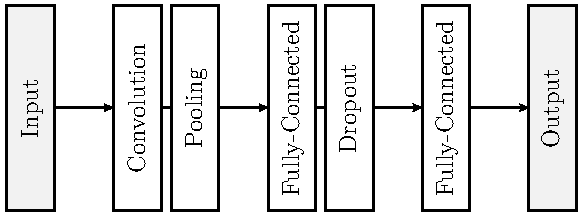
\includegraphics[]{images/cnn_layers.pdf}
	\caption[Layers of a convolutional neural network]{Layers of a convolutional neural network. Each combination of convolutional layer and pooling layer or fully-connected and dropout can be arbitrarily repeated. Moreover, pooling layers and dropout regularization layers are optional.}
	\label{fig:cnn-layers}
\end{figure}
Commonly, convolutional layers are combined with pooling layers and fully-connected layers with dropout regularization layers.
However, the latter combinations are optional.
Each of them is explained in the following sections.
Combinations and repetitions of those layers with their own hyperparameters are called architecture.
Usually, convolutional and pooling layers manipulate the input and the resulting activations before fully-connected layers appear.
There are different proposed architectures with their weights and biases available.
The most common ones are AlexNet \cite{Krizhevsky:2012:ICD:2999134.2999257}, VGG \cite{Simonyan15}, GoogLeNet \cite{szegedy2015} and, ResNet \cite{He2016ResNet}.

\input{tex/fundamentals/neural_networks/cnn/convolution.tex}
\input{tex/fundamentals/neural_networks/cnn/pooling.tex}
\input{tex/fundamentals/neural_networks/cnn/fully_connected.tex}
\subsection{Train a Neural Network}
\label{sec:neural-networks-training}
So far optimal weights and biases were assumed in all examples, that exactly model a desired function $f(\vec{x, \vec{W}, \vec{B}}) = \vec{y}$ where $\vec{W}$ and $\vec{B}$ store all parameters of a network.
But in practical terms, they need to be found first for generating the desired output.
This starts by collecting or generating and preparing a dataset from which the network can find correlations by changing the weights and biases.
Then, those parameters are randomly initialized.
Furthermore, the data samples of the dataset are used as input and are feed-forwarded through the network yielding a classification $\hat{\vec{y}}$.
This classification is evaluated by a cost function.
That result is back-propagated through the network by computing its gradients for changing the weights and biases.
The forward pass and backward pass are repeated with different samples until an termination condition is satisfied.
\figref{fig:training} illustrates this process.
Each of these steps is covered in the following sections.
\begin{figure}
	\centering
	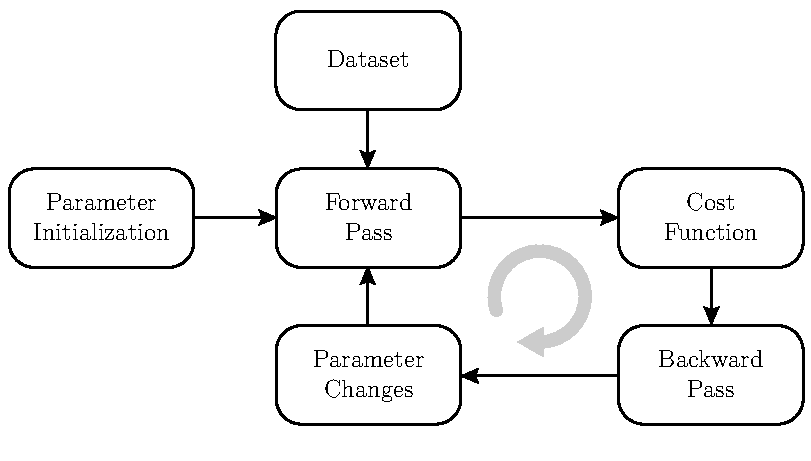
\includegraphics{images/training.pdf}
	\caption[Training process]{Training process. The parameters are initialized once at the beginning. The training process includes the forward pass, the cost function evaluation,the backward pass and the changing of parameters. This is repeated with different data samples.}
	\label{fig:training}
\end{figure}

\input{tex/fundamentals/neural_networks/training/dataset}
\input{tex/fundamentals/neural_networks/training/weight_initialization}
\input{tex/fundamentals/neural_networks/training/forward_pass}
\input{tex/fundamentals/neural_networks/training/gradient_descent}
\input{tex/fundamentals/neural_networks/training/adam}
\subsection{Improving Performance}
\label{sec:neural-networks-improving-performance}
Earlier sections make general recommendations on hyperparameters.
Nevertheless, there is room for improvement.
Finding well-suited hyperparameters is a trial-and-error method and requires much time.
However, there are methods that aim to find a good starting point.
Those are going to be presented in the following.

\input{tex/fundamentals/neural_networks/improving_performance/learning_rate.tex}
\input{tex/fundamentals/neural_networks/improving_performance/batch_size.tex}
\input{tex/fundamentals/neural_networks/improving_performance/activation_functions.tex}
\subsection{Metrics for Performance Evaluation}
\label{sec:neural-networks-metrics}
There are several common metrics available that, for example, measure the classification accuracy or its precision.
However, they depend on some definitions that will be introduced first.
The positive class of a data sample represents its ground-truth class, while the negative one represents any of the remaining ones, i.\,e. not the positive class.
A true positive $TP$ is a correct prediction of a sample, so the positive class is predicted correctly.
A true negative $TN$ is a correct rejection of a sample, i.\,e. the network classifies this sample correctly as not the positive class.
Furthermore, a false positive $FP$ is a wrong prediction of a sample as the positive class.
The last definition is a false negative $FN$.
This means the network incorrectly predicts a sample as a negative class.
Their connection is visualized in \figref{fig:confusion-matrix} showing the so-called confusion matrix \cite{Fawcett:2006:IRA:1159473.1159475} for the example class Class A.
This needs to be repeated for each class in a dataset.
\begin{figure}
	\centering
	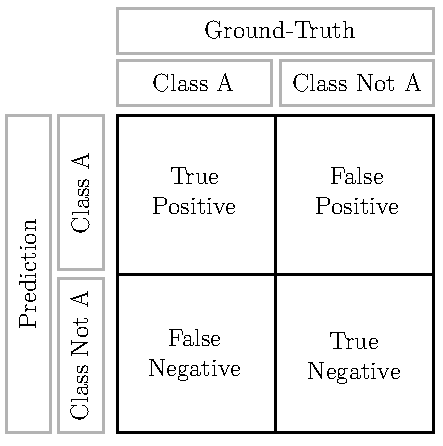
\includegraphics[]{images/confusion_matrix.pdf}
	\caption[Confusion matrix]{Confusion matrix for class A.}
	\label{fig:confusion-matrix}
\end{figure}
One metric is the accuracy
\begin{equation}
	ACC = \frac{TP + TN}{TP + TN + FP + FN}
\end{equation}
of a class.
Averaging all class accuracies yields the network accuracy.
This states how many samples the network correctly classifies.
However, this metric's results are not reliable for the real performance, because it highly depends on the dataset and its balance, among others.
If it is unbalanced there are, for example, more samples in a well-classifiable class than in a bad one, hence, the accuracy is shifted.
The precision or positive predicted value of a class measures how accurate the related predictions are and is calculated by
\begin{equation}
	\label{eq:metric-precision}
	PPV = \frac{TP}{TP + FP}
\end{equation}
where the denominator refers to the total positive results.
Furthermore, the recall or true positive rate metric measures how good all positives of a class are found by
\begin{equation}
	\label{eq:metric-recall}
	TPR = \frac{TP}{TP + FN}
\end{equation}
where the denominator refers to the actual positives of a class.
Both \eqref{eq:metric-precision} and \eqref{eq:metric-recall} must be calculated for each class to get a complete overview of the dataset.
A simplified representation of the confusion matrix can be prepared by entering only the number of predictions per class.
This is beneficial for a quick overview of the prediction distribution of multi-class classifications.
Similar to \figref{fig:confusion-matrix} each row represents a predicted class, while the columns represent the ground-truth classes.
Each prediction of the samples of a ground-truth class are summed per class and entered at the corresponding cell.
\section{Software}
This section focuses on explaining which software and frameworks are used for implementing the network and generating the dataset in this work.

\subsection{Tensorflow}
\label{sec:software-tensorflow}
Tensorflow is a free framework in particular for machine learning tasks.
It was originally developed by Google Brain for internal Google use and got finally licensed for open source. 
Mathematical operations are designed as a symbolic graph.
After its creation, any operation inside can be executed and only needs the computation of its dependent operations.
Every computation involves tensors.
A tensor is a generalization of scalars, vectors, and matrices independent on their dimension.
Hence, a definition of every tensor's size is important for a cost-effective creation and computation of the graph.
Due to the symbolic graph, it is possible to define a neural net with an input and output layer and steadily feed and compare different tensor values.
\subsection{Blender}
\label{sec:software-blender}
Blender \cite{blender} is a free and open source 3D creation suite to model, texture and animate objects.
Furthermore, it supports importing existing models and manipulating them.
Additionally, an API interface is provided, that can be used with the programming language Python, to control every function of Blender.
This eases repetitive tasks tremendously.

%Every object in Blender has its own coordinate system.
%Hence, a way of expressing points of one coordinate system in another would be useful.
%It is necessary to define a world coordinate system $\mathcal{W}$ with the origin $\vec{o}_\mathcal{W} = (0,0,0)^T$ and the rotation $\vec{r}_{\mathcal{W}} = (0,0,0)^T$, where each element of the latter represents a rotation around the $x$-, $y$- or $z$-axis, respectively, in radians.
%This system contains every other system.
%Now another coordinate system $\mathcal{L}$ is created, of course, inside the world coordinate system.
%However, $\mathcal{L}$ can be translated and rotated in comparison to $\mathcal{W}$.
%Hence, every coordinate system has a rotation matrix $\vec{R}$ in Euler representation and a translation vector $\vec{t}$ that stores how they are rotated and translated to every other coordinate system.
%Considering $\mathcal{L}$ and $\mathcal{W}$ yields
%\begin{align}
%	\vec{R}_{\mathcal{L} \rightarrow \mathcal{W}} &= \vec{R}_{\mathcal{W} \rightarrow \mathcal{L}}^{-1} \\
%	\vec{t}_{\mathcal{L} \rightarrow \mathcal{W}} &= - \vec{t}_{\mathcal{W} \rightarrow \mathcal{L}}
%\end{align}
%as properties, where the subscript indicates the transfer.
%Transferring the coordinates of an arbitrary local point $\vec{x}_{\mathcal{L}}$ into corresponding coordinates $\vec{x}_{\mathcal{W}}$ of the reference coordinate system is done by using
%\begin{equation}
%	\vec{x}_{\mathcal{W}} = \vec{R}_{\mathcal{L} \rightarrow \mathcal{W}} \cdot \vec{x}_{\mathcal{L}} + \vec{t}_{\mathcal{L} \rightarrow \mathcal{W}}
%\end{equation}
%as the general expression.
\chapter{Related Work}
\label{sec:related-work}
Earlier 3D shape descriptors were mostly handcrafted based on a particular geometric property of the actual shape's surface or volume.
Those descriptors can be divided into two groups.
On the one hand, there are model-based 3D descriptors, that are directly based on the available 3D representation of objects that have been modeled using polygons, voxels, or point clouds, among others.
\textit{Osada et al.} \cite{Osada:2001:MMS:882486.884103} describe the signature of 3D objects by their shape distribution sampled from geometric shape functions.
Those functions use angles, distances, areas and volumes of an object's polygon mesh for forming a shape distribution.
By comparing the shape distribution of an object with the ones from similar and dissimilar objects, the class of the current object is found.
On the other hand, there are view-based 3D shape descriptors.
Those are created using multiple 2D views of an object instead of the raw 3D representation.
\textit{Chen et al.} \cite{Chen2003} introduced LightField Descriptors, the first typical view-based descriptor.
Such a descriptor is created by capturing images from 20 cameras positioned at the vertices of a dodecahedron with the solid 3D object inside.
By assuming that the views remain in this spatial order, the descriptor of another object can be compared by rotating it, until both sets are aligned.
There are 60 different variants of aligning them.
For each variant the distance of both sets is calculated by comparing each view with its aligned one and adding the result up.
The comparison is based on the light field representing the radiance in each view.
The minimum distance of all variants is used for the classification.
\textit{Shu et al.} \cite{Shu:2016:MCV:2965260.2965467} presented the Principal Thickness Images Descriptor that describes contour and volumetric information of an object.
First, they voxelize a 3D mesh object and perform a principle component analysis for yielding the three principle directions of the object.
Then, they measure the thickness along those axes by counting the number of voxels along each.
The thickness is finally encoded into a gray-scale image for each axis where the intensity of a pixel represents the number of voxels along the related axis.
With the histogram of oriented gradients a feature descriptor for each image is extracted.
In general, the advantages of view-based shape descriptors are their low dimensionality compared to model-based ones and, hence, the efficiency for processing.
In general, view-based descriptors have desirable properties like low dimensionality and efficient evaluation.
Moreover, they are more robust to noisy or holey 3D representations.

With the introduction of convolutional neural networks like AlexNet \cite{Krizhevsky:2012:ICD:2999134.2999257} and their improvement in image classification, they could be used for creating descriptors.
This performance was further improved with famous architectures like VGG-Net \cite{Simonyan15}, ResNet \cite{He2016ResNet} and Inception-v4 \cite{SzegedyInceptionv4}.
According to the ImageNet challenge \cite{Russakovsky:2015:ILS:2846547.2846559} results, the last two architectures outperform humans regarding the top-5 classification error in 2D object classification.
Using a variation of the VGG architecture, the so-called VGG-M \cite{journals/corr/ChatfieldSVZ14}, \textit{Su et al.} \cite{Su:2015:MCN:2919332.2919750} make their eight-layer multi-view convolutional neural network, short MVCNN, learn a compact shape representation of the actual object by collecting information from any number of input views without a specific order.
Previous methods combine the information of views with simple strategies like pairwise comparisons of descriptors or concatenating descriptors from ordered, consistent views.
The MVCNN architecture, however, performs a maximum pooling operation across all views for collecting discriminative features in a single shape descriptor.
This leads to an accuracy of 89.9\,\%, which outperforms state-of-the-art descriptors, for a network trained on the ImageNet1k dataset \cite{Krizhevsky:2012:ICD:2999134.2999257} and fine-tuned with the ModelNet40 one \cite{conf/cvpr/WuSKYZTX15} with 12 views per object.
That means, the network is first trained with single views from ImageNet1k and further trained with multi-views from ModelNet40.
In contrast, learning a single-view classification with an identical training and fine-tuning yields an accuracy of 88.6\,\%.
In this case, the accuracies of the corresponding 12 views are averaged before the overall accuracy is calculated.
Moreover, MVCNN outperforms 3D ShapeNets \cite{conf/cvpr/WuSKYZTX15} that reaches an accuracy of 77.3\,\% and is using a convolutional network on raw CAD data.
Hence, it is trained with the ModelNet40 dataset.
In the comparison of 2D- and 3D-representations from \textit{Su et al.} \cite{Su2018} the MVCNN architecture outperforms architectures working on point clouds and voxels.
Furthermore, they could improve the performance of the vanilla MVCNN to 95.0\,\% per instance by using a deeper network and better object centering.
However, \textit{Hegde et al.} introduce their FusionNet \cite{Hegde2016FusionNet3O} that combines a multi-view architecture, in particular \cite{Su:2015:MCN:2919332.2919750}, with a volumetric convolutional neural network for achieving each representation's advantages.
The 2D-representation is used for local spatial correlations, while the 3D-representation is used for long-range spatial correlations.
Their architecture achieves an accuracy of 93.11\% on the ModelNet10 dataset with 20 views and 90.80\% on ModelNet40 with 60 views.
According to \textit{Feng et al.} \cite{Feng2018}, view-to-shape descriptor methods like the one from \textit{Su et al.} are a milestone for 3D shape recognition and reflect the state-of-the-art.
Since in \cite{Su:2015:MCN:2919332.2919750} all views are weighted equally, their goal is to exploit the discriminability among views and their intrinsic hierarchical correlation.
Hence, they add a module that divides views with similar features into the same group.
Views inside a group are mean pooled for creating a group descriptor for each group.
Furthermore, a group with more discriminative views is associated with a higher weight than groups with less discriminative views.
Finally, a single weighted group descriptor is computed representing the shape descriptor of the object.
Because the grouping mechanism sounds promising for helping evaluate the information content of views, in particular, the one of views of the same object but with different material color marks, this work is based on it.
Their network yields an accuracy of 92.6\,\% with an identical training and configuration as before and the GoogLeNet or Inception-v1 architecture \cite{szegedy2015}, respectively.
Using only 8 views results in an accuracy of 93.1\,\%.
With transferring the MVCNN concept to the GoogLeNet architecture, an accuracy of 92.2\,\% instead of 89.9\,\% is achieved.
Another view grouping approach is presented by \textit{Cyr et al.} \cite{Cyr2004} using handcrafted descriptors.
They define similarity metrics based on curve matching for performing the view grouping.
Because views are redundant in a large part they can be reduced to a minimal set.
They introduce the aspects graph representation.
The theory behind is, that a small change in the vantage point of an object results in only a small change in the view projection.
However, for some views that change is large.
Those views represent a transition, the views between an aspect.
Hence, it is supposed, that the first describes the object satisfiable.
\chapter{Methods}
\label{sec:methods}
This chapter explains the implementation of the neural network architecture for classifying objects and the generation and preparation of the dataset.
Each data sample used as an input for the network consists of multiple viewing perspectives of an object, a so-called multi-view.
Each object has duplicates, where a different color mark is applied to each copy.
The intention is to examine how the multi-view approach known from \cite{Su:2015:MCN:2919332.2919750} and, in particular, \cite{Feng2018} relates to multi-views where the shape of objects is the same but only differs in color marks.
Furthermore, it is analyzed how each view of a data sample contributes to the classification result.
In this context, the class of each object is referred to by a combination of its type of object and color mark.
Hence, the terminology category describes the first and color the latter.
The creation of the dataset is performed with the Blender API interface, while the model is written in Python using the tensorflow framework.

\section{Multi-View Network Architecture}
\label{sec:methods-architecture}
Researches showed that convolutional neural networks are well-suited for image classification tasks \cite{Simonyan15, He2016ResNet, SzegedyInceptionv4}.
Furthermore, in \cite{Su:2015:MCN:2919332.2919750} the VGG-M \cite{journals/corr/ChatfieldSVZ14} architecture is used for classifying multi-views.
This convolutional neural network uses eight layers and yields satisfying classification results for either single- or multi-views.
\textit{Feng et al.} \cite{Feng2018} show that the performance of this multi-view classification architecture can be improved by grouping views with similar informational content and weighting the groups accordingly.
A schematic of their group-view convolutional neural network architecture, short GVCNN, is illustrated in \figref{fig:gvcnn-framework}.
\begin{figure}
	\centering
	\includegraphics[width=\textwidth]{images/gvcnn_framework.png}
	\caption{Group-view convolutional neural network architecture (from \cite{Feng2018})}
	\label{fig:gvcnn-framework}
\end{figure}
Their architecture is based on GoogLeNet \cite{szegedy2015} and uses 22 layers.
Each view of a multi-view input is propagated through the same subset containing the first five main convolutional layers, labeled "FCN" in the figure, yielding a raw view descriptor for each.
Those are further propagated through the remaining main convolutional layers, labeled "CNN" in the figure, yielding a final view descriptor for each.
Based on those raw view descriptors a discrimination score for each view is calculated by propagating them through a fully-connected layer for dividing each view, in particular each final view descriptor, in groups.
Depending on the discrimination scores of all views in a certain group, this group is assigned a weight.
Furthermore, an inter-group view descriptor pooling yields a group descriptor for each group.
Combining all group descriptors depending on their weight, a final compact shape descriptor is generated that describes the shape of the object.
This is propagated through a final fully-connected layer, labeled "FC" in the figure, to get the classification result.

It is supposed that in particular the grouping process can be adapted to the task of distinguishing the same models with different color marks very well.
Furthermore, a view discrimination score supports the analysis of the information content of views.
Because the color mark is the only difference, the related views should be weighted the most while all others should only play a marginal role in the classification process.
This would reduce noise, thus, resulting in a better performance.
However, using the exact same architecture of GVCNN is not possible due to its number of parameters that exceeds the available resources for this work.
Hence, the AlexNet architecture \cite{Krizhevsky:2012:ICD:2999134.2999257} is chosen that consists of eight layers.
Regarding its layers it is very similar to the VGG-M but uses larger but less filters for convolutions and fewer nodes in the fully connected layers.
However, the less parameters are a trade-off for accuracy.
Because of the less layers compared to GVCNN the position of the generation of the view discrimination scores and the shape descriptor within the network is different.
The discrimination scores depend on the last main convolutional layer that is actually the fifth as well.
In MVCNN two of three fully-connected layers are used to generate a shape descriptor based on its single pooled view descriptor, while the third classifies it.
Based on this, each group descriptor is propagated through two fully-connected layers in this work's architecture for generating group shape descriptors.
Those are combined regarding their weights to a final, compact shape descriptor that is used for classification in the third fully-connected layer.

A summary of this work's architecture is presented in \tabref{tab:network-layers}.
Each layer's hyperparameters are explained in the following sections.
\begin{table}[]
\centering
\caption{Network layer summary}
\label{tab:network-layers}
	\begin{tabular}{lllll}
		Operation & Window       & Output Size                & Stride & Padding \\ \hline
		Conv1     & $7 \times 7$ & $109 \times 109 \times 96$ & 2      & Valid   \\
		Pool1     & $3 \times 3$ & $54 \times 54 \times 96$   & 2      & Valid   \\ \hline
		Conv2     & $5 \times 5$ & $27 \times 27 \times 256$  & 2      & Same    \\
		Pool2     & $3 \times 3$ & $13 \times 13 \times 256$  & 2      & Valid   \\ \hline
		Conv3     & $3 \times 3$ & $13 \times 13 \times 384$  & 1      & Same    \\ \hline
		Conv4     & $3 \times 3$ & $13 \times 13 \times 384$  & 1      & Same    \\ \hline
		Conv5     & $3 \times 3$ & $13 \times 12 \times 256$  & 1      & Same    \\
		Pool5     & $3 \times 3$ & $6 \times 6 \times 256$    & 2      & Valid   \\ \hline
		FcGroup   & 			 & 1					      &        &         \\ \hline
		Fc1       &              & 4096                       &        &         \\ \hline
		Fc2       &              & 4096                       &        &         \\ \hline
		Fc3       &              & \# of Classes              &        &         \\ \hline
		Softmax   &              &                            &        &         \\ \hline
	\end{tabular}
\end{table}
This work's network architecture is divided into three important modules as illustrated in \figref{fig:architecture-modules}.
The feature module takes all views of an object and calculates a descriptor for each.
Those are fed to the grouping module, that groups views dependent on their information content and outputs a descriptor for every group and additionally their weight.
Dependent on those outputs a single, compact descriptor is calculated, that describes the inputted shape or object, respectively, and is used for the classification.
Each of the modules is examined in detail in the following sections.
\begin{figure}
	\centering
	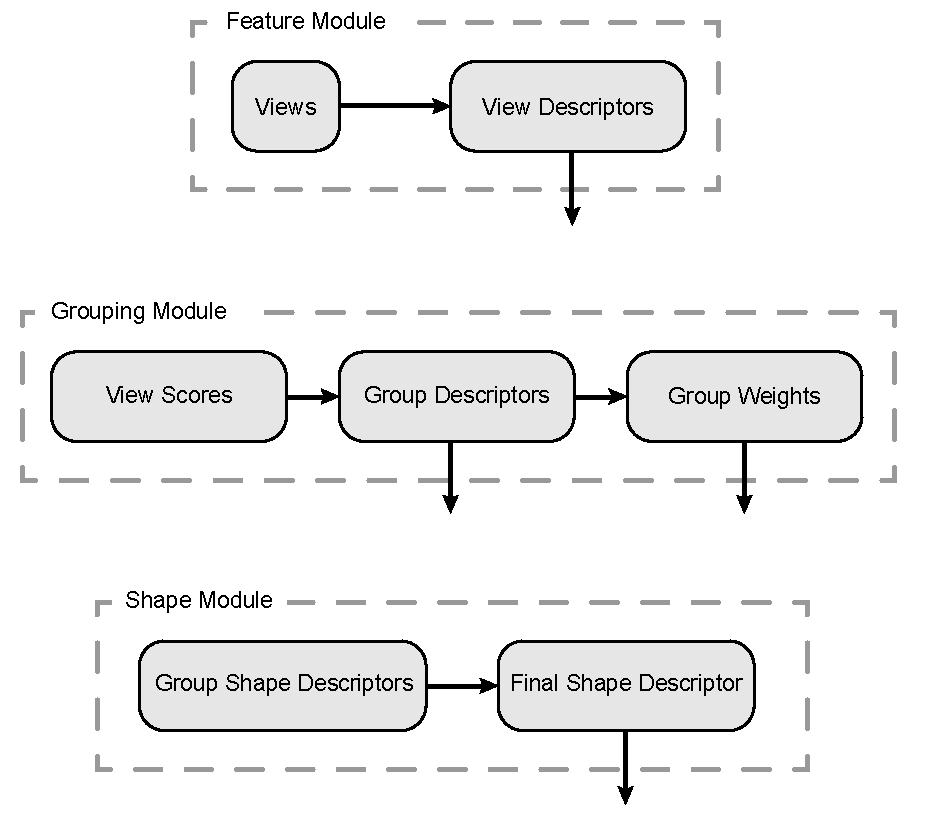
\includegraphics[]{images/multi_view_architecture.pdf}
	\caption{Modules of the multi-view architecture. The feature, grouping and shape modules are executed consecutively. Each module's operations are executed from left to right according their illustrated flow by arrows.}
	\label{fig:architecture-modules}
\end{figure}

\subsection{Feature Module: Generating View Descriptors}
\label{sec:architecture-feature-module}
The objective of the feature module is the generation of a descriptor for each view by using five convolutional layers.
Each one is referred to as a view descriptor $\vec{V}_i$ in the following.
\figref{fig:feature-module} shows the basic concept.
\begin{figure}
	\centering
	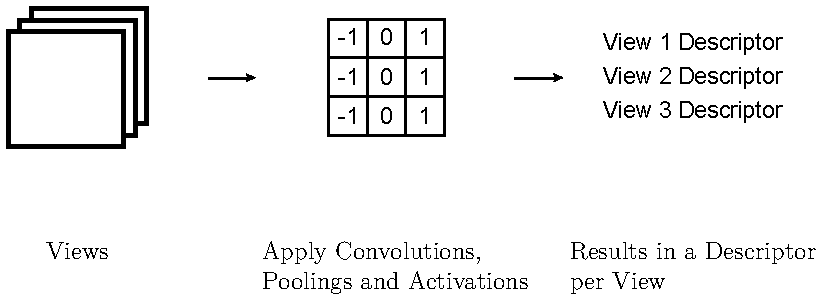
\includegraphics[]{images/feature_module.pdf}
	\caption{Basic Concept of the Feature Module}
	\label{fig:feature-module}
\end{figure}
This module is the first one in the feed-forward chain.
It is connected with the real world by having all views $\mathbb{V}$ of an object as its input.
Furthermore, because tensorflow supports batch execution, i.e. all its operations can be applied to a batch of data, the input tensor is extended with a batch dimension for multiple multi-views.
This yields an input tensor of shape $Batch \times Views \times Height \times Width \times Channels$.
In the following, if a tensor has a batch dimension, which is usually the case, it is assumed that any mentioned operation or approach is applied to every batch element.
This module consists of five main convolutional layers.
A main convolutional layer is supposed to have a convolutional layer and an optional pooling layer.
The first main layer performs a valid convolution with 96 filters of size $7 \times 7$ and a stride of 2 on each $224 \times 224 \times 3$ input.
Every filter extracts different features.
In comparison, the original AlexNet uses filters of size $11 \times 11$ and a stride of 4.
However, it is assumed that smaller filters and a smaller stride are collecting more information that can be used for a classification of the object and material at once.
A convolution operation is done by flattening the filter tensor to a 2D matrix of size $Filter\_Height \times Filter\_Width \times Channels\_In \times Channels\_Out$.
Here, $Channels\_in = 3$ because of the RGB channels of the input image and $Channels\_Out = 96$ because of the defined number of filters.
Then, image patches of shape $Batch \times Height\_Out \times Width\_Out \times Filter\_Height \cdot Filter\_Width \cdot Channels\_In$ are extracted from the input tensor.
Multiplying the filter matrix and the image patch vector yields the convolution results for the current window.
This is repeated for the whole input resulting in a matrix with a size of $1 \times 109 \times 109 \times 96$ in this case.
Furthermore, to each convolution output the corresponding bias is added.
This result is fed into a ReLU activation function.
Finally, the outputs are max-pooled with a window of size $3 \times 3$ and a stride of 2.
No padding is applied as well.
It is defined, that the max-pooling is always performed on the last dimension, i. e. the one containing each feature.
This yields a matrix of shape $1 \times 54 \times 54 \times 96$ for each convolution.
The next layers are similar including the bias addition and the ReLU activation function.
Hence, only the operations and their parameters will be mentioned.
Furthermore, the layers are added sequentially.
That means, the activations of the previous main layer are the input of the current main layer and so on.
The second main layer performs a convolution with 256 filters of size $5 \times 5$ and a stride of 2.
However, this time the input is padded in a way, that the output has the original input's size.
This yields a convolution result of shape $1 \times 27 \times 27 \times 256$.
The max-pooling uses again a window of $3 \times 3$ and a stride of 2.
The valid padding technique is applied resulting in a shape of $1 \times 13 \times 13 \times 256$.
The third and fourth main layer use 384 filters of size $3 \times 3$ for the convolution task with a stride of 1 each and the padding technique same.
However, no pooling is performed.
Hence, this yields a matrix of shape $1 \times 13 \times 13 \times 384$ both the times.
For the last main layer, the fifth one, a convolution with 256 filters of size $3 \times 3$ is performed.
The stride is 1 and the padding technique same, hence, the result has a size of $1 \times 13 \times 13 \times 256$.
The output's dimension is reduced with a valid max-pooling of size $3 \times 3$ and a stride of 2 to $1 \times 6 \times 6 \times 256$.
In the end, this whole process results in a tensor containing each view descriptor $\vec{V}_i$ of size $6 \times 6 \times 256$ of every batch element.
Hence, this tensor's shape is $Batch \times Views \times 6 \times 6 \times 256$.
\subsection{Grouping Module: Generating Group Descriptors}
\label{sec:architecture-grouping-module}
The objective of the grouping module is grouping each view descriptor $\vec{V}^{[5]}_v$ of an object depending on its information content.
This weights discriminative ones more than others, hence, improves the classification performance.
Moreover, based on each view's discrimination score an analysis of its information content is supported.
The view descriptors $\vec{V}^{[5]}_v$ of each group $\mathbb{G}_g$ are then combined to a group descriptor $\vec{G}_g$.
Hence, this module's inputs are the view descriptors coming from the feature module.
\begin{figure}
	\centering
	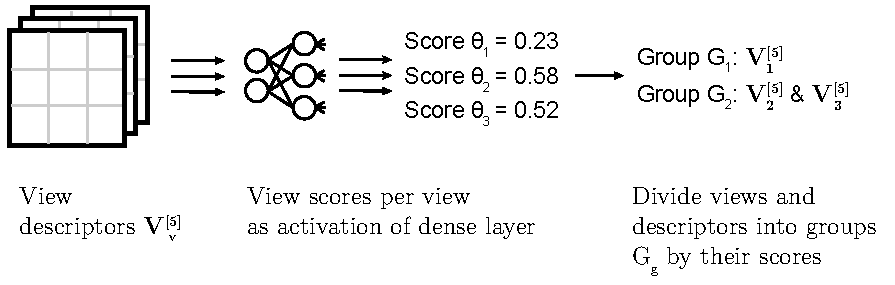
\includegraphics[]{images/grouping_module_groups.pdf}
	\caption{Group creation and view sorting in grouping module. Each view descriptor $\vec{V}^{[5]}_v$ is propagated through the same fully-connected layer yielding a view discrimination score $\theta_v$ based on which the view or view descriptor, respectively, is divided into a group $\mathbb{G}_g$.}
	\label{fig:grouping-module-groups}
\end{figure}
First, the informational content of each view needs to be calculated.
The simplest and most intuitive way is to give every view a single number representing its score of discrimination.
One approach would be to make the score directly depend on the pixel values.
This could be performed with a fully-connected layer with the pixels as inputs and the score as output.
However, like with fully-connected neural networks, this leads to many additional parameters for the network due to the translation-variance of input values. 
This could be overcome by using convolutions first for extracting features for the score.
However, discriminative features are already extracted, presumably much more accurate than a few convolutions for the score would do. 
Hence, the followed approach is that each view's score depends on its most recent descriptor $\vec{V}^{[5]}_v$.
It is worth noting, that in \cite{Feng2018} the view scores do not depend on the last convolution.
However, their network architecture uses more than five convolutional layers, but the scores depend on the fifth one as well.
This is probably because later features of deeper view descriptors are too detailed and would result in too divergent discrimination scores for a reliable group generation.
In this work's architecture each latest view descriptor $\vec{V}^{[5]}_v$ is fed into the same single fully-connected layer with one node.
Therefore, the view descriptor matrix is flattened into a row-wise vector, which is multiplied with the corresponding weight matrix $\vec{W}^{[d4]}$ of shape $6 \cdot 6 \cdot 256 \times 1$.
To this result a bias $b^{[d4]}$ is added yielding the weighted sum $z^{[d4]}$ with a single value.
This is fed into its activation function.
In contrast to every other layer in this network, a leaky ReLU activation function is applied to this unit.
A dropout is not performed, because with only one node it is not desirable.
Dropping out this node represents a view discrimination score of 0.
This would generalize the view scores way to strong, hence, unnecessarily extending training time.
Finding well-suited parameters for this layer would presumable take longer than for the others, thus, generating a bottle-neck in the architecture.
%It was found during training, that the unit died at the beginning of the training most of the time when using ReLU activation functions.
%This is due to its characteristic.
%If the weighted sum is zero or below at the beginning of the training due to an unsuited weight initialization, the activation is zero, hence, the neuron dies immediately.
%Another reason could be a too large learning rate, allowing the weights to update in too big steps leading to a weighted sum of 0 or below.
%This results in a view score of $0$ for every view that is not changed during later training steps due to a gradient of 0.
%The learning rate should suit the whole network and not only this layer, though.
%Their gradient is always unequal to zero, hence, it is solving the dying ReLU unit problem.

For interpretation purposes, the activation is squeezed into a range from 0 to 1 using the sigmoid function according to \cite{Feng2018} representing a probability of discrimination.
Because the sigmoid function saturates at values higher than around $\abs{5}$, but the activation of the fully-connected layer is assumed to be larger, the natural logarithm of the activation is computed first.
This shifts the saturation to values that are presumably not in the range of the activation.
For having a continuous function the absolute value of the activation is taken beforehand.
This yields the expression for a view's score
\begin{equation}
	\label{eq:view-discrimination-score}
	\theta_v = \sigmoid\left( \log \left( \abs{a^{[d4]}} + \varepsilon \right) \right)
\end{equation}
where $a^{[d4]}$ is the output or activation, respectively, of the corresponding fully-connected layer.
The small constant $\varepsilon=10^{-6}$ is added for numerical stability for avoiding $\log(0)$.
A plot of this function is shown in \figref{fig:view-discrimination-score}.
\begin{figure}
	\setlength\figureheight{.45\textwidth}
	\setlength\figurewidth{.8\textwidth}
	\centering
	\input{images/view_discrimination_score.tikz}
	\caption{View discrimination score function plot}
	\label{fig:view-discrimination-score}
\end{figure}
All view discrimination scores for a batch are stored in a tensor $\bar{\vec{\Theta}}$ with shape $Batch \times Views$.

Dependent on each view score, the related views or view descriptors, respectively, are divided into groups.
For maximum flexibility, the number of groups $n_g$ equals the number of views $n_v$.
Hence, the size of each group bin $r_{\text{bin}}$ is related to the number of views $n_v$ per object and the range of possible view scores $r_\theta$.
With the limit of \eqref{eq:view-discrimination-score}
\begin{equation}
	\lim_{a^{[d4]}\rightarrow \infty} \sigmoid\left( \log \left( \abs{a^{[d4]}} + \varepsilon \right) \right) = 1
\end{equation}
and only positive values from the ReLU, scores are in the range $r_\theta = 1 - 0 = 1$.
Dividing $r_\theta$ in equal sized parts yields
\begin{equation}
	r_{\text{bin}} = \frac{r_\theta}{n_v} = \frac{1}{12} \approx 0.083
\end{equation}
as each group bin's size related to the discrimination score values.
Hence, a group $\mathbb{G}_g$ contains view descriptors $\vec{V}_v^{[5]}$ of views with scores of $(g-1) \cdot r_{\text{bin}} \leq \theta_v < g \cdot r_{\text{bin}}$ where $g \in \{1,2, \dots, n_v\}$.
\figref{fig:grouping-module-groups} illustrates the basic view score calculation and grouping.
This example assumes a group size of $0.33$.
The group to which each view $\tilde{\vec{X}}^{(i)}_v$ belongs is calculated by
\begin{equation}
	g_v = \floor \left( \frac{\vec{\theta}_v}{r_{\text{bin}}} \right)
\end{equation}
yielding the group's index, where $\vec{\theta}_v$ is the view score of the $v$-th view of the corresponding multi-view sample.
Those are stored for every view resulting in the group index vector $\vec{g}_{\text{idx}} = \left( g_1, g_2, \cdots, g_{n_v}\right)^T$.
The subscripts correspond to the view indices, e.g. $g_2$ belongs to $\tilde{\vec{X}}^{(i)}_2$.
With this approach, it is possible for groups to remain empty.
Based on the group indices, related view descriptors are averaged across their first dimension.
In brief, every feature is averaged.
This is illustrated in \figref{fig:grouping-module-group-descriptors}.
\begin{figure}
	\centering
	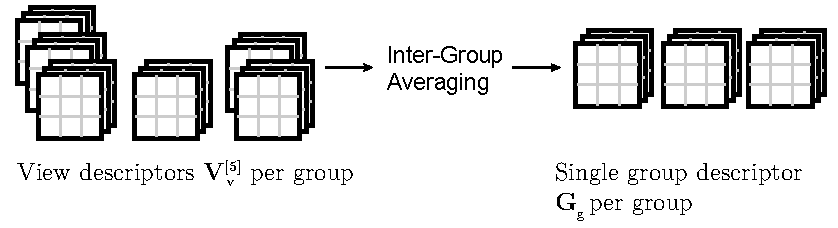
\includegraphics[]{images/grouping_module_group_descriptors.pdf}
	\caption[Generating group descriptors]{Generating group descriptors $\vec{G}_g$ by calculating the average of view descriptors $\vec{V}^{[5]}_v$ in each group $\mathbb{G}_g$.}
	\label{fig:grouping-module-group-descriptors}
\end{figure}
Because all view descriptors in a group should have similar extracted features, they can be combined by averaging them without a significant loss in information.
If the maximum of all features were taken, though, the group would presumably contain all view descriptors where important features were extracted for creating a group descriptor containing as many features as possible.
However, this is not desirable for the use case.
This results in a group descriptor
\begin{equation}
	\vec{G}_g = \frac{\sum_{\vec{D} \in \mathbb{G}_g} \vec{D}}{|\mathbb{G}_g|}
\end{equation}
with the same size as a view descriptor, where $\vec{D}$ is a view descriptor $\vec{V}_v^{[5]}$ of group $\mathbb{G}_g$.
The addition and division are calculated element-wise.
However, the views of different objects are not necessarily divided into the same number of groups, thus, leading to a different number of group descriptors.
For a valid matrix representation when using batches group descriptors of zero need to be added that the number of all batch's group descriptors match.
However, in the following $n_g$ is used for the group dimension for simplicity.
Hence, the final shape of the tensor $\bar{\vec{G}}$ containing all group descriptors is $Batch \times n_g \times 6 \times 6 \times 256$.

Every group $\mathbb{G}_g$ gets a weight $w_g$ assigned representing its discrimination.
This depends on the scores of its contained views.
Analog to before, views of a group are found by checking the group index vector $\vec{g}_{\text{idx}}$.
This time the related view scores are summed up and divided by their number for calculating a mean.
In mathematical terms,
\begin{equation}
	\hat{w}_g = \frac{\sum_{\vec{D} \in \mathbb{G}_g} \theta_v(\vec{D})}{|\mathbb{G}_g|}
\end{equation}
calculates the weight of the $g$-th group, where $\theta_v(\vec{D})$ is the score of a view descriptor $\vec{V}_v^{[5]}$ in $\mathbb{G}_g$.
Furthermore, the weight of a group is normalized by
\begin{equation}
	w_g = \frac{\hat{w}_g}{\max(\theta(\mathbb{G}_g))}
\end{equation}
to a range of 0 and 1, where $\max(\theta(\mathbb{G}_g))$ yields the maximum score of the given group, for being able to compare it with the ones in \cite{Feng2018}.
The calculation of the group weights is illustrated in \figref{fig:grouping-module-weights} referring to the example in \figref{fig:grouping-module-groups}.
\begin{figure}
	\centering
	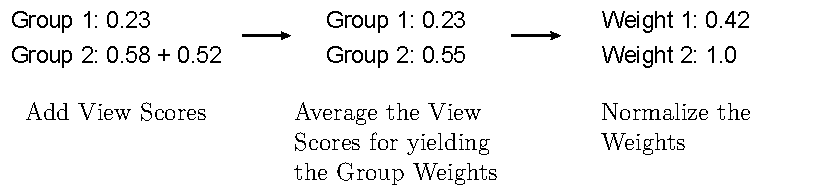
\includegraphics[]{images/grouping_module_weights.pdf}
	\caption{Calculation of group weights in grouping module}
	\label{fig:grouping-module-weights}
\end{figure}
All group weights of an object are stored in a vector $\vec{w}_{\text{groups}}$ of size $n_g$.
The corresponding tensor $\bar{\vec{W}}_{\text{groups}}$ has a size of $Batch \times n_g$.
\subsection{Shape Module: Generating a Shape Descriptor}
\label{sec:architecture-shape-module}
The objective of the shape module is to combine the group descriptors $\vec{G}_g$ of an object to a single shape descriptor that can be used for the classification.
All $n_g$ group descriptors of an object are stored in $\vec{G}$ that is of size $n_g \times 6 \times 6 \times 256$.
This descriptor contains every important feature of all views and groups.
Each group descriptor $\vec{G}_g$ is fed into a fully-connected sub-network with two layers.
The first layer has $6\cdot6\cdot256$ edges per unit and 4096 units in total, while the second layer has 4069 edges per unit and 4069 output units as well.
The inputs are processed like in the fully-connected layer before.
First, each input $\vec{G}_g$ is flattened into a column-vector $\vec{g}_g$.
Then, a matrix multiplication of the inputs and the corresponding weight matrix is performed and a bias vector is added.
This result is fed into a ReLU activation function $\phi(\cdot)$ resulting in an activation for the particular layer.
In conclusion, the two fully-connected operations
\begin{subequations}
	\begin{align}
		\vec{a}^{[6]}_g &= \phi(\vec{W}^{[6]} \vec{g}_g + \vec{b}^{[6]}) \\
		\vec{a}^{[7]}_g &= \phi(\vec{W}^{[7]} \vec{a}^{[6]}_g + \vec{b}^{[7]})
	\end{align}
\end{subequations}
are performed as illustrated in \figref{fig:shape-module-group-shape}.
\begin{figure}
	\centering
	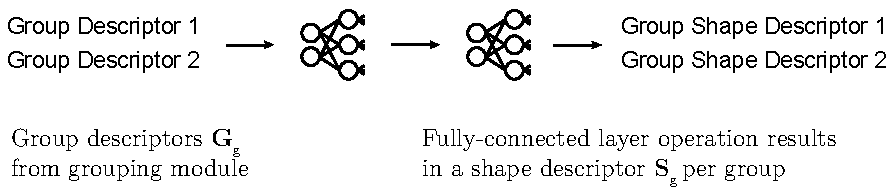
\includegraphics[]{images/shape_module_group_shape.pdf}
	\caption[Generate group shape descriptors in shape module]{Generate group shape descriptors in shape module. Each group descriptor $\vec{G}_g$ is propagated through two fully-connected layers representing layer 6 and 7 of the network. The activation of layer 7 represents the group shape descriptor $\vec{S}_g$ of each group descriptor.}
	\label{fig:shape-module-group-shape}
\end{figure}
Furthermore, both layers contain a dropout layer with a dropout probability of $0.5$.
This corresponds to the original AlexNet configuration.
Hence, the final activations of the seventh layer in the network or second dense layer, respectively, represent the shape descriptor of every group descriptor.
Those single group shape descriptor vectors of each group are and stacked along the second dimension to have a compact group shape descriptors representation $\vec{S}_{\text{groups}}$ with size $4096 \times n_g$.
Expanding this with a batch dimension yields the tensor $\bar{\vec{S}_{\text{groups}}}$ with size $Batch \times 4096 \times n_g$.

Now the group shape descriptors need to be combined for generating the final single shape descriptor of the object.
This is done by considering the corresponding group weights $\vec{w}_{\text{groups}}$ with $n_g$ elements calculated in the grouping module.
As a reminder, they are the mean of all view scores of each group, thus, an indicator for the group's discrimination.
Hence, a weighted average is calculated for considering this relation.
For this calculation the sums of the weights in inevitable.
Thus, $w_{g,\text{sum}}$ stores the sum of the group weights of an object.
The weighted average can be computed by
\begin{equation}
	\vec{s} = \frac{\vec{S}_{\text{groups}} \vec{w}_{\text{groups}}} {w_{\text{groups},\text{sum}}}
\end{equation}
where the division is performed element-wise.
The result has a shape of $4096$ and represents the final single shape descriptor.
The related assembled tensor $\bar{\vec{S}}$ has the size $Batch \times 4096$.

This representation is directly compatible with the last fully-connected layer, which is responsible for calculating the predictions of the network, thus, $\vec{s}$ is fed into it.
The number of neurons in this layer equals the number of classes where each neuron has 4096 edges.
The performed operations are identical to the ones earlier and are described by
\begin{equation}
	\vec{z}^{[8]} = \vec{W}^{[8]} \vec{s} + \vec{b}^{[8]}
\end{equation}
using the related weights and biases.
However, no activation function is applied here.
For making the predictions $\vec{z}^{[8]}$ interpretable, they are fed into a softmax layer.
This outputs a valid probability distribution $\hat{\vec{y}}$ depending on all its inputs $\vec{z}^{[8]}$.
Hence, this results in a membership probability for the network's input for each class.
The class representing the index with the largest value in $\hat{\vec{y}}$ is considered the predicted class. The functionality of the shape module is summarized in \figref{fig:shape-module-final-shape}.
\begin{figure}
	\centering
	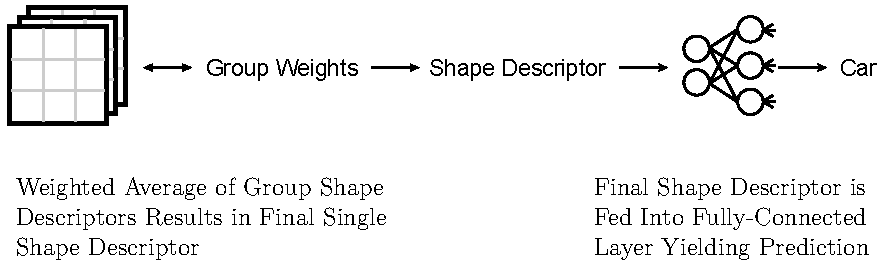
\includegraphics[]{images/shape_module_final_shape.pdf}
	\caption[Basic concept of the shape module]{Basic concept of the shape module combined with a classification. A weighted average of the group shape descriptors $\vec{S}_{\text{groups}}$ with the related group weights $w_{\text{groups}}$ is calculated yielding a single shape descriptor $\vec{s}$. It is fed into the last fully-connected layer resulting in the prediction $\hat{\vec{y}}$ of the network.}
	\label{fig:shape-module-final-shape}
\end{figure}
\section{Dataset Generation}
\label{sec:methods-dataset-generation}

\subsection{Choosing a Dataset}
\label{sec:dataset-choosing}
One requirement of the dataset is, that there are multiple views of the same object available.
Optimally, these views can be arbitrarily chosen for having as much freedom as possible for training and evaluating the network.
Hence, three-dimensional objects are necessary.
The related object categories are preferably discriminative to each other due to the objective of classifying real-world objects and easier evaluation of the model.
This means the dataset should not contain only flowers or faces for example.
These constraints bring up two possibilities.
The first one is creating new CAD objects.
These can be modeled in a way that supports the own needs the most.
However, creating plenty of models for every category would take a huge amount of time.
The second option is to use CAD models of an existing dataset.
Referring to the first possibility, this one just takes the time for finding a suited dataset and perhaps some slight modifications.
The time for manipulating this one according to the wanted color features compared to the self-created one is probably identical and, therefore, not taken into account.
Another advantage is the competitive ability because if this one is a popular dataset, other researches probably used it as a benchmark for their neural network as well.
Hence, a qualitative evaluation would be possible.
Taking all these arguments into account, an existing dataset is the best choice.

There are three different techniques for building a three-dimensional shape.
One uses triangles, where each one is defined by the position of its edges.
These positions are called vertices and contain an $x$-, $y$- and $z$-coordinate.
Additionally, each triangle has a normal vector and other information like a color and a texture.
Combining several triangles results in the final shape that is called a mesh object.
Another one uses voxels.
This word is a portmanteau of "volume" and "pixel" and represents a cell in a three-dimensional grid.
Each voxel behaves like a pixel and has a color.
The last technique is the point cloud.
Each point is represented by a vertex.
Such a cloud is often created by 3D scanners that measure a large number of points in a scene, like distances and sometimes color for digitalizing it.
A comparison of these techniques yields that the mesh object is the best-suited one.
It has the smoothest surface because it is continuous, hence, representing real-world objects most likely.
Using enough voxels could result in a similar shape, but the data size would be much bigger.
Furthermore, applying a color feature to a single triangle is easier than applying it to several voxels, where connected ones need to be found first.

The most popular dataset containing CAD objects in polygon mesh representation is ModelNet\cite{conf/cvpr/WuSKYZTX15}.
It contains 127,915 CAD models divided into 662 object categories for now.
For convenience, there are a 10-class and 40-class subset containing 10 or 40 popular categories, respectively.
Both are cleaned in respect to a wrong category sorting and then split into a training and a testing set.
Furthermore, the orientations of the models of the first one are aligned as well.
\subsection{Rendering Views of CAD Models}
\label{sec:dataset-rendering}
The following explains how multiple viewing perspectives of a single model are generated.
The properties of each CAD model of ModelNet are stored in a file that is loaded and interpreted in Blender.
To be able to refer to faces they are all part of the same basic coordinate system and are placed according to their defined vertices.
Because all models are oriented beforehand, their top points along the $z$-axis.
The origin of this coordinate system is set to the center of mass depending on the face areas.
For adding lighting to the object a lamp needs to be placed inside that coordinate system.
Blender offers several lamp types, but the Hemi lamp was chosen because it emits light radially from a plane.
Therefore, a homogeneous illumination is ensured.
%\begin{figure}
%	\centering
%	\begin{subfigure}{0.19\textwidth}
%		\centering
%		\includegraphics[width=\textwidth]{images/point.png}
%		\caption{Point}
%	\end{subfigure}
%	\begin{subfigure}{0.19\textwidth}
%		\centering
%		\includegraphics[width=\textwidth]{images/sun.png}
%		\caption{Sun}
%	\end{subfigure}
%	\begin{subfigure}{0.19\textwidth}
%		\centering
%		\includegraphics[width=\textwidth]{images/spot.png}
%		\caption{Spot}
%	\end{subfigure}
%	\begin{subfigure}{0.19\textwidth}
%		\centering
%		\includegraphics[width=\textwidth]{images/hemi.png}
%		\caption{Hemi}
%	\end{subfigure}
%	\begin{subfigure}{0.19\textwidth}
%		\centering
%		\includegraphics[width=\textwidth]{images/area.png}
%		\caption{Area}
%	\end{subfigure}
%	\caption[Lamp types available in Blender]{Lamp types available in Blender. Each light source is placed above the cube pointing directly towards it.}
%	\label{fig:blender-lamps}
%\end{figure}
Because all models have different heights and this type of lamp has no decay of intensity, it is placed above the objects far away from their origins.
By assigning the lamp a direction $\vec{r}_l = (0,0,0)^T$ it emits light along the negative $z$-axis directly onto the model.

For rendering views, a camera object is required.
Its parameters are left to the default values, except its view distance, which is set very high to work with all models.
Hence, only its location and rotation needs to be set.
Following the approach from \cite{Su:2015:MCN:2919332.2919750, Su2018} the camera is elevated 30 degrees from the ground plane and points towards the origin.
This results in the first rotation vector
\begin{equation}
	r_{c,0} = \left( \frac{r_{x,\text{deg}} \cdot \pi}{180}, 0, 0 \right)^T = \left( \frac{60 \cdot \pi}{180}, 0, 0 \right)^T
\end{equation}
in radians, where $r_{x,\text{deg}}$ is the rotation around the $x$-axis in degrees.
The first, second and third element define a rotation around the $x$-, $y$- and $z$-axis, respectively.
Because the camera points along the negative $z$-axis in its own coordinate system by default, $r_{x,\text{deg}} = 60$ corresponds to the mentioned setup.
The next step is fitting the camera view to the model just by changing the location of the camera.
Because Blender fits the camera view exactly to the object, an image padding is necessary for having empty border regions for later convolutions.
This is achieved by moving the camera away from the object along the line of their centers, i.\,e. along the negative view direction.
It is moved by
\begin{equation}
	\Delta d = \frac{d}{10}
\end{equation}
where $d$ is the distance from the mesh origin to the camera.
The advantage of a fraction is, that the padding is independent of the model's size.
Finally, this camera view is rendered with the following properties.
The resolution is defined to be $224 \times 224$ pixel
Furthermore, it needs to be coped with aliasing.
Because every pixel can only have a single color, diagonal lines usually have a step pattern.
This is not realistic, hence, it is smoothed out by anti-aliasing techniques.
This works by rendering the related image region in a higher resolution, taking several samples of pixel values and averaging them to get the value of the pixel in the desired resolution.
The best available sample size in Blender is 16, hence, it is chosen.
The background color is left at the default RGB color $\vec{c} = (64, 64, 64)$ resembling a dark gray for adding some noise to the views.
A black background would yield pixel intensities of 0 and resembles, in general, no real-world views.
Finally, this view is saved as a PNG file.
For gathering multiple views, the camera needs to be repositioned.
Hence, the following steps are repeated for the desired number of views.
The rotation of the camera is set to
\begin{equation}
	\vec{r}_c(v_i) = \left(  \frac{60 \cdot \pi}{180}, 0, \frac{v_i \cdot \varphi \cdot \pi}{180} \right)^T
\end{equation}
where $v_i$ is the view index, originally starting at 0, and $\varphi$ the moving interval in degrees.
The latter is set to
\begin{equation}
	\varphi = \frac{360}{n_v} = \frac{360}{12} = 30
\end{equation}
where $n_v$ equals the number of views.
For the ability to compare this work to related researches, $n_v = 12$ is defined.
The number of objects per set corresponds to \cite{Su:2015:MCN:2919332.2919750}.
That means, 90 objects per category class for the training set and 30 for the test set.
This process is repeated for each CAD object.
\subsection{Applying Material Feature Manipulations}
\label{sec:dataset-material-feature}
The objective is to clone every model and apply a color feature to every clone to be able to distinguish the same models.
Cloning is a trivial task because this can be done by rendering the native object first and then the color featured one.
One method for the color feature manipulation is preparing a color feature like a colored circle as an image and putting it on the model.
This feature can be scaled dependently on all the face areas for achieving a similar scale across all models.
However, clinging this image to a model considering all its edges is problematic.
It would be necessary to find a way to unfold the model along its edges.
This can be done by hand but is very time-consuming and complex.
In fact, Blender supports an automatic way of unfolding, but its results are not satisfying.
Therefore, this approach is not further pursued.
Another method is to color vertices.
However, for achieving reasonable features, a high number of vertices is necessary.
There is an option to subdivide existing faces and add additional vertices, but this increases the data size extremely, which needs much more computer performance and has the risk of inducing unwanted geometry into the model.
Hence, coloring single faces becomes the chosen approach due to its simplicity.
In CAD modeling objects are assigned a material with a color that reacts to light which produces shadows.
In Blender, the default material's color is a slightly darkened white.
Changing the color of a face is performed by changing the color of its material.

For following this approach, it is advisable to pre-define material presets.
Those presets consist of the default material but have different colors.
After making those presets available to the Blender scene, a well-suited face for being colored needs to be found.
In the following those faces are referred to as an optimal face.
It is important to filter all faces of an object by their area size.
\figref{fig:face-area-filter} shows why and the results of several thresholds.
\begin{figure}
	\centering
	\begin{subfigure}{.32\textwidth}
		\centering
		\includegraphics[width=\textwidth]{images/face_area_unfiltered.png}
		\caption{Unfiltered}
		\label{fig:face-area-unfiltered}
	\end{subfigure}
	\begin{subfigure}{.32\textwidth}
		\centering
		\includegraphics[width=\textwidth]{images/face_area_mean.png}
		\caption{Face Area Mean}
		\label{fig:face-area-mean}
	\end{subfigure}
	\begin{subfigure}{.32\textwidth}
		\centering
		\includegraphics[width=\textwidth]{images/face_area_max_dependent.png}
		\caption{Max Face Area Dependent}
		\label{fig:face-area-max-dependent}
	\end{subfigure}
	\caption{Threshold Setup for Filtering Faces by their Area Size}
	\label{fig:face-area-filter}
\end{figure}
If faces are not filtered at all, any face can result in being the optimal one.
However, it is not guaranteed that this face has a decent size and can be seen and recognized by the network easily.
This assumption was later verified by a not changing loss value during training.
Like in \figref{fig:face-area-unfiltered} the optimal face is comparatively small to the whole model.
Accepting only faces as the optimal face, that have at least the size of the mean of all faces lead to a result like in \figref{fig:face-area-mean}.
The optimal face can be seen more easily than before, but this threshold often results in long and slender optimal faces.
This is due to the fact, that the chosen object categories mostly contain objects that are built using such faces because they have longish surfaces.
Hence, filtering by the mean of the faces amplifies the probability to choose such a face as an optimal one.
Therefore, a threshold of above the mean is desired to skip all those lathy faces like it is shown in \figref{fig:face-area-max-dependent}.
Additionally, larger faces should be preferred.
Thus, the area of the optimal face have to satisfy
\begin{equation}
	a_{opt} > (a_{mean} + a_{max}) \cdot s
\end{equation}
where $a$ are the related areas and $s$ a scalar.
With $s = 0.3$ satisfying results are achieved.

Furthermore, it needs to be guaranteed, that the optimal face is visible in at least one view and not visible in at least one view.
This is validated by casting rays from the camera center onto the possible optimal face for every camera position that was defined in \secref{sec:dataset-rendering}.
In brief, if the rays hit the face, the face is visible.
Fortunately, there is a function in Blender performing this approach and returning among others the index of the face that is hit.
However, this cannot be performed for every pixel of a face due to performance issues.
Thus, the trade-off against accuracy is only checking the vertices defining the face.
This can raise errors, though, because a vertex can define multiple faces and it is not certain which face index the function returns.
Hence, each checkpoint $\vec{p}_i$ is moved slightly to the center of the face by
\begin{equation}
	\vec{p}_i = \vec{v}_i + 0.05 \cdot (\vec{f}_0 - \vec{v}_i)
\end{equation}
where $\vec{v}_i$ is the related vertex and $\vec{f}_0$ the center of the face.
If the ray cast is valid for at least one checkpoint the face is supposed to be visible.
If all rays hit the wrong face, the current face is supposed to be not visible.
As soon as both conditions are satisfied for the examined face among all views, it becomes the optimal face.
Otherwise, the next possible face is investigated.
If the conditions are never satisfied for each possible face, the object is skipped at all.

It is found, that a single optimal face is not enough, because some models have several duplicated faces.
Those are different faces where the coordinates of all the describing vertices are identical to the ones of other faces.
Hence, there are faces laying into each other.
This results in rendering issues like it is shown in \figref{fig:optimal-face}, because the rendering engine does not know, which material should be rendered on the surface.
In \figref{fig:optimal-face-single} only one of two identical faces is colored, which leads to the noticeable transparency effect.
That is one of the brighter effects, though.
It is also possible that one optimal face is shown normally and only on the edge rendering issues are visible like a dotted line with the colors of all optimal faces. 
Nevertheless, any of these effects could induce false correlations into the dataset that are not available on real-world objects, hence, leading to a not practical network.
Thus, in \figref{fig:optimal-face-all} the materials of all identical faces are changed, which leads to realistic color representations.
\begin{figure}
	\centering
	\begin{subfigure}{.49\textwidth}
		\centering
		\includegraphics[width=.7\textwidth]{images/optimal_face_single.png}
		\caption{Single Optimal Face}
		\label{fig:optimal-face-single}
	\end{subfigure}
	\begin{subfigure}{.49\textwidth}
		\centering
		\includegraphics[width=.7\textwidth]{images/optimal_face_all.png}
		\caption{All Optimal Faces}
		\label{fig:optimal-face-all}
	\end{subfigure}
	\caption{Material Manipulation on Duplicated Optimal Faces}
	\label{fig:optimal-face}
\end{figure}

Regarding a validation of the later model, an examination of two material features per object would be interesting.
Hence, for applying another material change on a model, another optimal face or faces, respectively, needs to be found.
A requirement for this is the presence of only one material feature in a single view.
Due to the automation of this task, a reliable solution is necessary.
One approach would be using the other side of the surface of the first optimal face.
However, this fails if the surface has a thickness of more than a single face.
Then the next face along its normal needs to be found by ray casting and then the visibility of this face needs to be verified.
Thus, this process leads to excessive ray cast validations and therefore not followed up on.
However, it is considered, that faces at a similar location as the original optimal face are well-suited as well.
Thus, the choices of further optimal faces are narrowed down by sorting all remaining faces by their distance from their center to the center of the first optimal face in descending order.
The intention is that choosing faces with the largest distances result in either a kind of opposite face or in a face that is that far away to not be visible at the same time. as the first optimal face.
Of course, the tasks of checking the visibility and finding identical faces are performed on the new face as well.
If no additional optimal face is found, the model is skipped, although, this never happened during execution.
\section{Preparing the Dataset}
\label{sec:methods-prepare-data}

\subsection{Single-View to Multi-View Conversion}
\label{sec:prepare-data-view-conversion}
The objective of the network is to classify multi-views of objects.
This means each input represents an object with all its corresponding views.
However, the views created in \secref{sec:dataset-material-feature} exist in single view representation because they are rendered successively.
Thus, each model's single views need to be converted into a related multi-view representation.
For achieving this, all single views are collected in order of their creation for keeping their relation.
Each view's pixel values are read, normalized to a range between 0 and 1, flattened to a vector $\vec{x}^{(i)}$ and stored in the input matrix $\vec{X}_{\text{set}}$ of the corresponding set.
Simultaneously to the view gathering each one-hot encoded label $\vec{y}^{(i)}$ needs to be created as well and put into the label matrix $\vec{Y}_{set}$ of the corresponding set similar to the views.
Each label may contain an object class, the so-called category, and a color mark class, the so-called color.
Depending on the type of classification, these two classes possibly need to be combined.
The single-label classification case embraces the following configurations.
If categories and colors are classified, both classes are appended to each other.
This results in $n_y = n_c \cdot n_m$ classes for classification, where $n_c$ is the number of categories and $n_m$ the number of color marks.
If only categories or color marks are classified, the final label contains only the category class or the material class, respectively.
Logically, the number of classes for classification, is either $n_y = n_c$ or $n_y = n_m$.
In the multi-label classification case, both labels are used independently.
Hence, the number of classes for classification equals $n_y = n_c + n_m$.
An example of those configurations is shown in \tabref{tab:label-generation}.
\begin{table}[]
	\centering
	\caption[Label generation]{Label generation with example category classes "bathtub" and "sofa" and color mark classes "0" and "1" for different cases of classifications.}
	\label{tab:label-generation}
	\begin{tabular}{l|l|l}
		Classification      & Single-Label                                                                        & Multi-Label                                                    \\ \hline
		Category + Material & \begin{tabular}[c]{@{}l@{}}bathtub\_0\\ bathtub\_1\\ sofa\_0\\ sofa\_1\end{tabular} & \begin{tabular}[c]{@{}l@{}}bathtub\\ sofa\\ 0\\ 1\end{tabular} \\ \hline
		Category            & \begin{tabular}[c]{@{}l@{}}bathtub\\ sofa\end{tabular}                              & n/a                                                            \\ \hline
		Material            & \begin{tabular}[c]{@{}l@{}}0\\ 1\end{tabular}                                       & n/a                                                           
	\end{tabular}
\end{table}
When the number of classes is known, a one-hot encoding is performed on each label.
Dividing each input and output matrix into datasets yields
\begin{subequations}
	\begin{align}
		\label{eq:dataset-train}
		\mathbb{D}_{\text{train}} &= \left( \vec{X}_{\text{train}}, \vec{Y}_{\text{train}} \right) \\
		\label{eq:dataset-test}
		\mathbb{D}_{\text{test}} &= \left( \vec{X}_{\text{test}}, \vec{Y}_{\text{test}} \right)
	\end{align}
\end{subequations}
where each column of $\vec{X}$ and $\vec{Y}$ of the same set are building an input-output pair.

Those single view and label representations need to be converted to a multi-view representation yielding $\tilde{\vec{X}}_{\text{set}}$ and $\tilde{\vec{Y}}_{\text{set}}$, respectively.
Because sorted data was read in, it is known that each $n_v=12$ elements belong together and need to put together somehow.
Looking at common definitions yield, that images are a three-dimensional matrix with the shape definition $Height \times Width \times Channels$.
Furthermore, tensorflow mostly uses the shape definition $Batch \times Height \times Width \times Channels$ for tensors.
Hence, reshaping each view back to a matrix representation of its original size and assuming it as a batch element is a reasonable approach for generating a multi-view of an object.
If an actual batch dimension becomes necessary it is inserted as a new first dimension.
Because each $n_v$ labels are identical, it is sufficient to just keep every $n_v$-th label for the multi-view representation.
For a later lookup of the labels, they are saved to the disk as a text file.
\section{Training the Architecture}
\label{sec:methods-training}
This work's multi-view network architecture is trained by inputting the generated multi-view images $\tilde{\vec{X}}_{train}^{(i)}$ and comparing the prediction $\hat{\vec{y}}^{(i)}$ of the network with the corresponding label $\tilde{\vec{y}}_{train}^{(i)}$.
First, a batch size needs to be chosen to define how many samples will be fed to the network at once.
In a training using only single-views, a batch size of 128 could be achieved.
Thus, using $n_v = 12$ views the batch size is reduced to $m_b = floor(128 / 12) = 10$.
However, due to a limited memory size of 8GB of the experimental setup's GPU and the additional parameters for the multi-view training only a batch size of 8 supports training reliably.
This yields $n_{b,train} = m_{train} / 8$ batches for the training set and $n_{b,test} = m_{test} / 8$ for the test set.
Nevertheless, dividing each set into 8 samples will be odd in general.
Thus, the last batch is filled with all the remaining samples.
After each epoch, the training set is shuffled randomly, so that batches do not contain the same samples as before.
For simplicity, a sample in the shuffled list is still referred to by its current index.

For calculating the cost and the derivatives of the parameters a softmax cross entropy is performed in the single-label classification case.
For efficiency, tensorflow applies a softmax internally, so the unscaled predictions need to be fed.
Then, the softmax measures the probability error between the prediction and ground-truth labels, while assuming mutually exclusive classes.
In the multi-label classification case, sigmoid cross entropy is applied.
Here the sigmoid is calculated internally and not mutually exclusive classes are assumed.
For updating the parameters with the goal of minimizing the cost function the Adam optimizer is employed due to its advantages.

The predictions $\hat{\bar{\tilde{\vec{Y}}}}^{(i)}$ of the network need to be compared to the ground-truth labels $\bar{\tilde{\vec{Y}}}^{(i)}$ of the $i$-th batch for checking the network's accuracy.
Due to the batch operations, the single dataset samples in a batch are referred to as batch samples.
How the comparison is performed, though, depends on the type of classification.
In the case of a single-label one, the index of the largest value in the batch element prediction $\hat{\tilde{\vec{y}}}^{(i)}$ is located.
The same operation is performed on the corresponding ground-truth label $\tilde{\vec{y}}^{(i)}$.
Each index represents a certain class, which is declared the predicted or actual one, respectively.
Now a binary comparison of both indices is performed, resulting in 0 if they are different and 1 if they are equal.
This is repeated for each batch element while storing all results in a tensor $\bar{\vec{E}}^{(i)}$.
Finally, the prediction accuracy $\alpha_{\text{p}}^{(i)}$ of the $i$-th batch is calculated by
\begin{equation}
	\label{eq:accuracy-mean}
	\alpha_{\text{p}}^{(i)} = \frac{\sum_{j} \bar{E}_j^{(i)}}{\left|\bar{\vec{E}}^{(i)}\right|}
\end{equation}
for the current batch $i$.
In the case of multi-label classification, a probability threshold needs to be defined when a predicted feature is actually considered predicted.
In this case, the threshold is $p_{\text{thres}}=0.5$, hence, the values of the prediction vector can be rounded.
Now an identical binary comparison as before can be applied to both label vectors resulting in a tensor $\bar{\vec{E}}^{(i)}$ as well.
The prediction accuracy is calculated with \eqref{eq:accuracy-mean}.

Furthermore, an initial learning rate is necessary.
Because finding it by trial-and-error would be time-consuming, the approach of the cyclical learning rate is used for finding an optimal learning rate.
The learning rate is initialized with $\gamma = 10^{-5}$.
After processing each batch it is exponentially increased according to
\begin{equation}
	\gamma(\tau+1) = \lambda \gamma(\tau)
\end{equation}
where $\lambda = 1.1$ is the scaling factor and $\tau$ the iteration.
Its value can be chosen arbitrarily but should be in range for achieving a desirable precision in learning rates.
For each learning rate, the related cost function evaluation is stored.
Training is stopped when the current cost value is four times the second to last one, i.\,e. when a drastic deterioration in cost happens, for having a noticeable oscillating characteristic at the end.
For evaluation, the cost values are plotted against the learning rates.
On the basis of this, the range of optimal learning rates can be read where a steep descent in cost values happen.
Optimally, this must be performed for each different network architecture.
\section{Evaluating the Architecture}
\label{sec:methods-evaluate}
For a comprehensive analysis of the network architecture of this work, especially the grouping mechanism and the information content of views, a lot of data has to be collected.
Fortunately, every tensor can be gathered and, if necessary, manipulated to be interpretable.
The most important tensor for training contains the cost of every iteration of the training set because this is attempted to be minimized, because it represents how well the network classifies the data.
Each one is stored during training to be able to plot them afterwards.
Furthermore, after each epoch, the cost and accuracy of the whole training and test set are calculated with current parameters.
Because the ModelNet10 dataset is split by default only into a training and test set, the latter is used additionally as a validation set.
The cost and accuracy of each set is computed by computing them for each batch and averaging the results.
However, the last batch has in general fewer elements than the ones before.
Hence, a weighted average is performed with the batch sizes as the weights.
This yields the averaged cost
\begin{equation}
	J\left(\hat{\bar{\tilde{\vec{Y}}}}, \bar{\tilde{\vec{Y}}}\right) =  \frac{\sum_{i}^{n_b} m_{b_i} \cdot J\left(\hat{\bar{\tilde{\vec{Y}}}}^{(i)}, \bar{\tilde{\vec{Y}}}^{(i)}\right)}{\left|\vec{m_b}\right|}
\end{equation}
and the averaged prediction accuracy
\begin{equation}
	\alpha_\text{p}\left(\hat{\bar{\tilde{\vec{Y}}}}, \bar{\tilde{\vec{Y}}}\right) =  \frac{\sum_{i}^{n_b} m_{b_i} \cdot \alpha_\text{p}\left(\hat{\bar{\tilde{\vec{Y}}}}^{(i)}, \bar{\tilde{\vec{Y}}}^{(i)}\right)}{\left|\vec{m_b}\right|}
\end{equation}
where $\vec{m_b}$ is a vector containing the batch sizes.
As mentioned, this is performed separately on the training set and the test set.
Those results are also stored for plotting purposes.
Comparing both related units can reveal if training should be continued or if overfitting or underfitting occurs.
Because the cost value is more general and the accuracy rather for practical purposes, the first one is examined.
If the training loss decreases while the training loss decreases as well, the network improves and training should be continued.
However, if the training loss decreases while the test loss increases, overfitting is indicated.
The network does not generalize, but focuses on the features in the training set, hence, never seen data like the test set cannot be classified properly.
At the end of the training, the accuracy of the training set is defined as the performance of the network.
To plots, whose shown values $\vec{\omega}$ oscillate, a moving average $\vec{\Omega}$ of the values is added.
A single averaged value is calculated by
\begin{equation}
	\Omega_i = \frac{\sum_{j = \max(1,i-\eta+1)}^{i} \omega_j}{\max(0,i-\eta)}
\end{equation}
where $\eta$ is the window size, that defines how many values are taken into account for averaging a certain sample.
If the window is larger than the available number of samples, in particular in the beginning, the window size is adapted temporarily.
By default it is set to $\eta=\floor\left( 0.1 \left| \vec{\omega} \right| \right)$ for a dynamical size.

For evaluating the whole network model regarding its practical use, the accuracies for each class, each category, and each color are calculated separately.
That means for the second and third, that each category accuracy includes all related multi-views independent of color and each color class accuracy includes all related multi-views independent of the category.
In general, the accuracy states how many samples are classified correctly.
However, the overall accuracy can be misleading, although each class has almost the same number of objects because it does not represent if certain classes are better classified than others.
Hence, the precision and recall score is computed for each class as well.
Furthermore, a simplified confusion matrix is calculated containing every sample's prediction.
It is plotted against the ground-truth classes, where predictions of identical classes are counted up.
The grouping module needs to be evaluated as well.
It is supposed that in a classification of only the color, the views with visible color manipulations belong to the highest weighted group.
Hence, it is sufficient to examine if the most discriminative group only contains views with visible manipulations.
Because the colors of the manipulated faces are known, each pixel of a view in the top group is checked if it matches such an RGB value.
If there is a match with at least one pixel of a view, the view is considered grouped correctly.
All correctly grouped views $TP$ and not correctly grouped views $FP$ are counted.
Based on them a percentage
\begin{equation}
	\label{eq:metric-group}
	\alpha_{\text{precision}}^{(i)} = \frac{{TP}^{(i)}}{{TP}^{(i)} + {FP}^{(i)}}
\end{equation}
is calculated representing the precision of the grouping module for a given multi-view input $i$.
This is repeated for all multi-views of the same color.
The final precision for that color results from averaging the precision of every multi-view of that color and is considered its group metric.
This is performed for every color to analyze if different colored face manipulations yield different results. 

For predicting the classes and gathering information of certain inputs, multi-views of objects need to be given.
These build a common input tensor $\bar{\tilde{\vec{X}}}^{(i)}$ representing the $i$-th batch.
If the number of samples, that are going to be predicted, exceeds the defined batch size, they need to be divided into an appropriate number of batches.
This tensor is now propagated through the network as usual.
%Meanwhile, the activations of the first convolutional layer are stored for visualizing the extracted features in each view.
%Therefore, each view's activations are split across the last dimension that represents the features.
%Each feature's values $\vec{F}_i$ are normalized by
%\begin{equation}
%	\label{eq:normalize}
%	\vec{F}_{i,norm} = \frac{\vec{F}_i - \min(\vec{F}_i)}{\max(\vec{F}_i) - \min(\vec{F}_i)} 
%\end{equation}
%to a range of 0 and 1 for making it visualizable.
%Finally, each feature is saved as an gray-scale image.
Meanwhile, each view discrimination score, group weight, and group index is stored for showing them with their associated view afterwards.
%Furthermore, a saliency map $\vec{S}_v^{(i)}$ is computed for each view $\tilde{\vec{X}}_v^{(i)}$ showing how much each pixel influences the raw output of the network $\vec{z}^{(i)}$.
%Here, the direct output of the eighth layer is taken, that means no softmax is applied.
%A single saliency map can be defined as the derivative of the output with respect to a single view yielding
%\begin{equation}
%	\label{eq:saliency-map}
%	\vec{S}_j^{(i)} = \frac{\partial \vec{z}^{(i)}}{\partial \tilde{\vec{X}}_v^{(i)}}
%\end{equation}
%as a general expression.
%For plotting each saliency map is normalized with \eqref{eq:normalize} and visualized in gray-scale.
\chapter{Results}

\section{View to Group Classification}
\label{sec:results-grouping}
Because the grouping mechanism supplies the core functionality of the network architecture it is evaluated first.
Even if the overall performance would yield satisfiable results, but the grouping mechanism would fail the original intention, it would need to be revised.
In contrast, if the results of the network are not satisfiable, the grouping algorithm could be the cause.

The easiest case for evaluation is a single object category with three material features.
Here the network only needs to find views with a material for assigning them a high discrimination score.
It is supposed, that those views have the highest scores of all views and, hence, are members of a group with a high weight.
Views where no material is seen, should have a score close to zero, because the final prediction cannot rely on them at all.
Thus, this configuration is the most interpretable one.
The group dividing for the 0-3 network is shown in \figref{fig:grouping-0-3}.
Each number below a view refers to its score.
The text above views shows the group index with its corresponding weight.
All views appear in a ascending order by their score.
Hence, all subsequent views are part of a group until another group is mentioned.
\begin{figure}
	\centering
	\begin{subfigure}{\textwidth}
		\includegraphics[trim=10 20 10 20, clip]{images/mn-sl-0-3-20/bathtub_0107_0_grouping.png}
		\caption{Blank}
		\label{fig:grouping-0-3-blank}
	\end{subfigure}
	\begin{subfigure}{\textwidth}
		\includegraphics[trim=10 20 10 20, clip]{images/mn-sl-0-3-20/bathtub_0107_1_grouping.png}
		\caption{Green Material}
		\label{fig:grouping-0-3-green}
	\end{subfigure}
	\begin{subfigure}{\textwidth}
		\includegraphics[trim=10 20 10 20, clip]{images/mn-sl-0-3-20/bathtub_0107_2_grouping.png}
		\caption{Red Material}
		\label{fig:grouping-0-3-red}
	\end{subfigure}
	\caption[Grouping in 0-3 Network]{Grouping in 0-3 Network}
	\label{fig:grouping-0-3}
\end{figure}
In \figref{fig:grouping-0-3-blank} a blank object is classified.
Hence, every views is similar discriminative, due to no available colored material.
Thus, the view scores are almost identical.
Those little changes presumable depend on a different weight initialization and would even out after more training epochs.
Although the scores are very low, the views are fully taken into account because they all belong to the same group with a weight of 1.
However, in this particular case a normalization of the group weight is not necessary.
Without one the group weight would be $w = 0.0079$, thus, decreasing the shape descriptor enormously, but the network would learn that a descriptor close to 0 represents a blank object.
The decision rule would be, if the descriptor represents no feature, the objects shows no feature.
With the classification of more categories, tough, this is not possible anymore, because a very small descriptor cannot just represent any blank object, but the object category class.
If there are two objects, for example, and only one view each shows a different feature with a small discrimination score, they would be divided into two categories.
Without a normalization all views would pretty much account to the same amount to the shape descriptor.
With normalization, however, the group with one view is much higher weighted than the not discriminative views.
Hence, normalization kind of removes noise, i.e. not discriminative views, that could influence the prediction unfavorably.
\figref{fig:grouping-0-3-green} and \figref{fig:grouping-0-3-red} show the expected result.
The views showing the material feature are by far the top rated views referring to their score.
It looks like, that the network prefers the slightly tilted vertical edge with a feature to its right for recognizing material features.
This exact edge is not visible in the first view showing a feature, due to the change in perspective.
Due to the mesh representation of objects, all material features are triangles.
Perhaps the dataset contains more features following this shape than in rotated ones, hence, the network focuses on that correlation.
Moreover, both figures show exactly the same order.
This shows, that the weights for each color channel are optimized in the same direction.
However, the views with the green material are in a closer range compared to the ones with the red material.
The latter differ extremely.
The least discriminative view with a material is closer to the not discriminative views than the discriminative ones.

%It is supposed, that similar views like opposite perspectives of a symmetrical object are divided into the same group, because they contain similar features.
%For example, the views of the left and right side of a car look almost identical.
%Both have the same contours but in a mirrored direction.
\section{Overall Performance}
\label{sec:results-overall}
\section{Misclassified Predictions}
\label{sec:results-predictions}
\chapter{Discussion}
\label{sec:discussion}
\section{Conclusions}
\label{sec:discussion-conclusion}
The objective of this work is to classify objects using multi-views.
In particular the same objects are classified but with different applied color marks.
Furthermore, the information content of these multi-views is analyzed and how views with different color marks impact this and the actual classification.
This basic network architecture of \textit{Feng et al.} \cite{Feng2018} is used, that assigns views a discrimination and groups them accordingly.
This is manipulated by using the AlexNet architecture with a modified first convolutional layer.
Moreover, the view discrimination scores are placed at a different position in the network.
Furthermore, for each group a group shape descriptor is generated that are then combined to yield the final, compact shape descriptor that is used for classification.
This architecture yields satisfiable results with respect to its loss and accuracy.
Because it is trained with a subset of ModelNet10, a direct comparison with recent researches is not possible.
However, the closest network for comparison with the MVCNN and GVCNN is 4-0 because it classifies only objects and no color marks.
This network's test accuracy is 99.4\,\%, while MVCNN reaches 89.9\,\% and GVCNN 92.6\,\%.
However, the 4-6 network is competitive with 85.5\,\%.

The grouping mechanism shows that, in particular, with the addition of color classes the network gets more complicated, hence its loss increases and its accuracy decreases.
It is noticeable, that using 5 or 6 color classes, wrong predictions are very likely to be within the same category class but with the related single or double color mark of the same color.
This can presumably be coped by a larger dataset or a longer training due to no indicator of overfitting.
Furthermore, it is observed across all networks that presumably ranges of values in the final shape descriptor are defined that correspond to color classes.
The assumed hierarchy starts with blank color classes as the highest values.
This is followed by red, red-red, green, green-red and green-green.
In general, views showing no color mark are more discriminative than views showing one, because the network uses them for excluding color classes from its possible predictions.
In practical terms, this means, for example, that a robot does not necessarily need to capture an entire object in order to make an accurate prediction.
\section{Outlook}
\label{sec:discussion-outlook}
The current networks can be improved by tuning the dataset among others.
More lights could be added to the scene or the current light is placed at the position of the camera and points along its view axis directly at the object.
This way more shadows are created in a view presumably leading to a detection of more edge features.
For creating optimal faces that are not occluded by others, ray casts for as many vertices in the face as possible need to be performed and checked if the ray hits the actual face.
However, this gets very computational expensive and would take a huge amount of time.
The advantage of this would be, that those results could be stored an used for finding the second optimal face.
If resources and time are no constraints, every other face could be examined for being the second optimal face.
Its results are then compared with the ones from the first one under the restriction of a given number of views where one should be visible.
Otherwise, choosing a valid face with the maximum distance from the first is a working approach.
In this case, though, a manual deleting of some bad samples needs to be performed.
Furthermore, the trained networks could be tested on real-world samples.
Real-world objects could be digitalized with a 3D scanner and propagated through the network.
This is likely to give somehow different results as true 3D models.
Moreover real world colors and materials can be assigned to each model, either CAD or digitalized, for supplying more features.

The networks could be improved by a longer training because no indication of overfitting exists.
Moreover, restarts for the learning rate could be added to avoid the differences in loss for the four-category networks by stepping over small minima.
Furthermore, a change in number of groups and their bin size could be evaluated.
However, it cannot be rated if this improves the performance.
The minimum of groups should be related to the current number of groups used for the predictions, though.
Probably the largest boost in performance would be a change of the underlying network architecture.
There are many networks that achieve higher accuracies according to the ImageNet challenge in object detection in images like Inception-v4 and ResNet.
If they are combined with the grouping mechanism higher accuracies than with the current implementation are expected.
However, the position of the grouping module and the input of the fully-connected layer for calculating the view discrimination scores are different if the new architecture is nested.
Their properties need to be examined first.


%\appendix			% schaltet Umgebunsvariablen um auf Anhang
%\input{appendix1}		% erster Teil des Anhangs (wird eher selten benötigt)

\backmatter			% Literaturverzeichnis, Index usw.

%%%%%%%%%%%%%%%%%%%%%%%%%%%%%%%%%%%%%%%%%%%%%%%%%
% Literatur
%%%%%%%%%%%%%%%%%%%%%%%%%%%%%%%%%%%%%%%%%%%%%%%%%
\begingroup
\raggedright\sloppy
\bibliography{literature}		% Name der *.bib Datei in der die Literatur steht
\endgroup
%\nocite{*}						% Auflisten aller Quellen, auch wenn diese nicht in der Arbeit zitiert sind

% Stil des Literaturverzeichnis (nach DIN1505)
%\bibliographystyle{unsrtdin} % sortiert nach Reihenfolge im Text mit Nummern
\bibliographystyle{enplaindin} % alphabetisch sortiert mit Nummer
%\bibliographystyle{alphadin} % alphabetisch sortiert mit Autor-Jahr-Kürzel statt Nummer

\end{document}
